%=============================================================================
% FloodEye - Internship Project Report
% Main driver file: compile with pdflatex (run twice for ToC/refs)
%=============================================================================
\documentclass[12pt,a4paper,oneside]{report}

%--------------------------------------------------------------
% Packages
%--------------------------------------------------------------
\usepackage[T1]{fontenc}
\usepackage[utf8]{inputenc}
\usepackage{lmodern}
\usepackage[top=2.5cm,bottom=2.5cm,left=3cm,right=2.5cm]{geometry}
\usepackage{microtype}
\usepackage{setspace}
\onehalfspacing
\usepackage{amsmath,amssymb}
\usepackage{graphicx}
\usepackage[table,xcdraw,dvipsnames]{xcolor}
\usepackage{float}
\usepackage{tikz}
\usetikzlibrary{shapes.geometric,arrows.meta,positioning,fit,backgrounds,shadows,calc}
\usepackage{pgfplots}
\pgfplotsset{compat=1.18}
\usepackage{booktabs}
\usepackage{longtable}
\usepackage{array}
\usepackage{tabularx}
\usepackage{multirow}
\usepackage{listings}
\usepackage{fancyhdr}
\usepackage{emptypage}
\usepackage[colorlinks=true,linkcolor=NavyBlue,citecolor=NavyBlue,urlcolor=NavyBlue,bookmarksnumbered=true,pdftitle={FloodEye Internship Project Report},pdfauthor={Moharnab Gogoi; Aryyaman Bora; Mayuree Khanikar; Indrani Gogoi}]{hyperref}
\usepackage{bookmark}
\usepackage[labelfont=bf,font=small,skip=6pt]{caption}
\usepackage{subcaption}
\usepackage{enumitem}
\usepackage[bottom]{footmisc}
\usepackage{titlesec}

%--------------------------------------------------------------
% Colors
%--------------------------------------------------------------
\definecolor{FloodBlue}{HTML}{1D4ED8}
\definecolor{FloodTeal}{HTML}{0891B2}
\definecolor{FloodGray}{HTML}{64748B}
\definecolor{FloodLight}{HTML}{EFF6FF}
\definecolor{CodeBg}{HTML}{F8FAFC}
\definecolor{CodeKeyword}{HTML}{1D4ED8}
\definecolor{CodeString}{HTML}{166534}
\definecolor{CodeComment}{HTML}{6B7280}

%--------------------------------------------------------------
% Chapter/section titles
%--------------------------------------------------------------
\titleformat{\chapter}[display]{\normalfont\huge\bfseries\color{FloodBlue}}{\chaptertitlename\ \thechapter}{12pt}{\Huge}
\titlespacing*{\chapter}{0pt}{0pt}{24pt}
\titleformat{\section}{\normalfont\Large\bfseries\color{FloodBlue!80!black}}{\thesection}{1em}{}
\titleformat{\subsection}{\normalfont\large\bfseries\color{FloodGray}}{\thesubsection}{1em}{}
\titleformat{\subsubsection}{\normalfont\normalsize\bfseries\color{FloodGray}}{\thesubsubsection}{1em}{}

%--------------------------------------------------------------
% Header/Footer
%--------------------------------------------------------------
\setlength{\headheight}{14pt}
\pagestyle{fancy}
\fancyhf{}
\fancyhead[L]{\small\textit{FloodEye: Real-time Flood Alert \& Water Level Monitoring}}
\fancyhead[R]{\small\thepage}
\fancyfoot[C]{\small\textcolor{FloodGray}{Technology Innovation Hub, IIT Guwahati}}
\renewcommand{\headrulewidth}{0.4pt}
\renewcommand{\footrulewidth}{0.4pt}

%--------------------------------------------------------------
% Code listings
%--------------------------------------------------------------
\lstset{
  backgroundcolor=\color{CodeBg},
  basicstyle=\ttfamily\footnotesize,
  keywordstyle=\bfseries\color{CodeKeyword},
  stringstyle=\color{CodeString},
  commentstyle=\itshape\color{CodeComment},
  numberstyle=\tiny\color{FloodGray},
  numbers=left,stepnumber=1,numbersep=8pt,
  showstringspaces=false,breaklines=true,breakatwhitespace=true,
  frame=single,framerule=0.4pt,rulecolor=\color{FloodBlue!30},
  tabsize=2,captionpos=b,
  xleftmargin=12pt,xrightmargin=4pt,aboveskip=8pt,belowskip=8pt,
}
\lstdefinelanguage{TypeScript}{
  keywords={const,let,var,function,async,await,return,export,import,from,interface,type,class,extends,new,this,if,else,for,while,switch,case,break,default,null,undefined,true,false,try,catch,finally,throw,void},
  sensitive=true,comment=[l]{//},morecomment=[s]{/*}{*/},
  string=[b]",morestring=[b]',morestring=[b],
}

%--------------------------------------------------------------
% TikZ styles
%--------------------------------------------------------------
\tikzset{
  process/.style={rectangle,rounded corners=6pt,draw=FloodBlue,fill=FloodLight,text width=3.2cm,minimum height=0.9cm,align=center,font=\small\bfseries},
  iotbox/.style={rectangle,rounded corners=6pt,draw=FloodTeal,fill=FloodTeal!10,text width=3.2cm,minimum height=0.9cm,align=center,font=\small\bfseries},
  arrow/.style={-{Stealth[length=6pt]},thick,color=FloodBlue},
  arrowg/.style={-{Stealth[length=6pt]},thick,color=FloodGray},
  startend/.style={ellipse,draw=FloodBlue,fill=FloodBlue!15,text width=2.4cm,minimum height=0.8cm,align=center,font=\small\bfseries},
  wideproc/.style={rectangle,rounded corners=6pt,draw=FloodBlue,fill=FloodLight,text width=4.5cm,minimum height=0.9cm,align=center,font=\small\bfseries},
}

\newcommand{\colorrule}{\vspace{4pt}\noindent\textcolor{FloodBlue!40}{\rule{\linewidth}{0.6pt}}\vspace{4pt}}

%=============================================================================
% DOCUMENT
%=============================================================================
\begin{document}

\pagenumbering{roman}
%=============================================================================
% Chapter 0: Cover Page — Clean Professional Theme
%=============================================================================
\begin{titlepage}
\newgeometry{top=2.5cm,bottom=2.5cm,left=2.5cm,right=2.5cm}
\thispagestyle{empty}

% Logos row
\begin{center}
  
\includegraphics[height=1.8cm]{../public/logotih.png}
  \hspace{3cm}
  
\includegraphics[height=1.8cm]{../public/iitlogo.png}
\end{center}

\vspace{0.8cm}

\begin{center}
  {\large\bfseries\color{FloodBlue!80!black} INTERNSHIP PROJECT REPORT}\\[0.2cm]
  {\normalsize\color{FloodGray} Technology Innovation Hub, IIT Guwahati}
\end{center}

\vspace{1.2cm}

\begin{center}
  {\fontsize{48}{55}\selectfont\bfseries\color{FloodBlue} FloodEye}\\[0.4cm]
  {\Large\bfseries\color{FloodBlue!75!black} Real-time Flood Alert \&\ Water Level Monitoring System}\\[0.5cm]
  \textcolor{FloodTeal}{\rule{8cm}{1.2pt}}\\[0.4cm]
  {\normalsize\itshape\color{FloodGray} ``Every Drop Monitored, Every Life Protected.''}
\end{center}

\vfill

\begin{center}
  \renewcommand{\arraystretch}{1.6}
  \begin{tabular}{@{} >{\bfseries\color{FloodBlue}}r @{\hspace{1em}\textcolor{FloodTeal}{\textbullet}\hspace{1em}} l @{}}
    Project Domain      & IoT, Machine Learning \& Web Dashboard \\
    Organisation        & Technology Innovation Hub (TIH), IIT Guwahati \\
    Duration            & 2 July 2026 -- 29 July 2026 \\
    Mentor              & Mr.\ Ashish Kumar Mahato \\
    Date                & 29 July 2026 \\
  \end{tabular}
\end{center}

\vfill

\begin{center}
  {\Large\bfseries\color{FloodBlue!80!black} Team Members}\\[0.5cm]
  \renewcommand{\arraystretch}{1.2}
  \setlength{\tabcolsep}{1.5cm}
  \begin{tabular}{cc}
    % Row 1 — names
    \textcolor{FloodBlue}{\textbf{\large Moharnab Gogoi}}
      & \textcolor{FloodBlue}{\textbf{\large Aryyaman Bora}} \\
    % Row 1 — roles
    \textcolor{FloodGray}{\itshape IoT Backend \& Cloud}
      & \textcolor{FloodGray}{\itshape Frontend \& UI Engineering} \\[0.4cm]
    % Row 2 — names
    \textcolor{FloodBlue}{\textbf{\large Mayuree Khanikar}}
      & \textcolor{FloodBlue}{\textbf{\large Indrani Gogoi}} \\
    % Row 2 — roles
    \textcolor{FloodGray}{\itshape Documentation \& Research}
      & \textcolor{FloodGray}{\itshape Documentation \& Research} \\
  \end{tabular}
\end{center}

\restoregeometry
\end{titlepage}
\clearpage

\thispagestyle{empty}
\vspace*{5cm}
\begin{center}
  {\Large\bfseries\color{FloodBlue!80!black} Live Dashboard Access}\\[0.8cm]
  
  The FloodEye live dashboard can be accessed at:\\[0.3cm]
  \Large \url{https://iot-tih.vercel.app/}\\[0.6cm]
  
  \normalsize
  The source code repository is available on GitHub at:\\[0.3cm]
  \Large \url{https://github.com/EnderMRG/IOT-TIH}\\[1cm]
  
  \normalsize
  \textbf{Demo Credentials:}\\[0.4cm]
  \renewcommand{\arraystretch}{1.5}
  \begin{tabular}{>{\bfseries}l l}
    Admin Email: & \texttt{admin@floodeye.com} \\
    Admin Password: & \texttt{Admin@FloodEye123!} \\[0.3cm]
    User Email: & \texttt{user@floodeye.com} \\
    User Password: & \texttt{User@FloodEye123!} \\
  \end{tabular}\\[1.5cm]
  
  \textcolor{red}{\textbf{Important Note:}} If the website does not open while connected to the IIT Wi-Fi network, please switch to a personal internet connection.
\end{center}
\clearpage


\tableofcontents
\listoffigures
\listoftables

\clearpage
\pagenumbering{arabic}

%=============================================================================
% Chapter 1: Introduction
%=============================================================================
\chapter{Introduction}

\section{Background}

Flooding is one of the most frequent and destructive natural disasters affecting millions of people globally, and the Indian subcontinent — in particular the Brahmaputra river basin of Assam — is among the most vulnerable regions in the world. Each monsoon season, rapidly rising water levels inundate vast agricultural tracts, damage infrastructure, displace communities, and claim lives. Historically, disaster response in these regions has been reactive: by the time human observers detect an unsafe water level and communicate the warning to downstream communities, the available evacuation window is dangerously narrow.

The convergence of Internet of Things (IoT) sensor technology, real-time cloud data platforms, and modern machine learning has created a new class of early warning systems that can operate continuously, inexpensively, and at the network edge. Instead of relying on manual gauge readings or expensive government-operated stations, a low-cost ESP32 microcontroller equipped with environmental sensors can upload telemetry to the cloud every 15 seconds, 24 hours a day, feeding an intelligent dashboard that monitors conditions, generates alerts, and predicts water levels up to four hours in advance.

\textbf{FloodEye} is a response to this need: a full-stack Progressive Web Application (PWA) developed during the internship at the Technology Innovation Hub (TIH), IIT Guwahati, that brings together IoT hardware, cloud integration, a modern web frontend, and an in-browser machine learning model into a cohesive, deployable flood early warning system.

\section{Problem Statement}

Despite the widespread availability of affordable IoT components and cloud platforms, most rural and semi-urban monitoring deployments in flood-prone regions suffer from one or more of the following deficiencies:

\begin{itemize}[leftmargin=1.5em]
  \item \textbf{Manual data collection:} Water level gauges require physical inspection, introducing delays and gaps.
  \item \textbf{No predictive capability:} Existing simple telemetry dashboards display only current readings; they cannot forecast whether levels will reach dangerous thresholds in the next several hours.
  \item \textbf{No offline resilience:} If the network link to a sensor breaks, many dashboards simply show an error, losing even the last known reading.
  \item \textbf{High infrastructure cost:} Dedicated server deployments for prediction models require significant maintenance overhead not feasible for research or municipal teams.
  \item \textbf{Poor user experience:} Many monitoring tools present raw JSON feeds or rudimentary tables rather than actionable, visually clear information.
\end{itemize}

FloodEye was designed to address every one of these gaps using modern, open, and cost-effective technology.

\section{Existing Challenges}

Several technical and operational challenges were encountered that shaped the design of FloodEye:

\begin{enumerate}[leftmargin=1.5em]
  \item \textbf{Sensor data latency:} The ESP32 uploads to ThingSpeak every 15 seconds; the dashboard must cache data intelligently to avoid serving stale readings while preventing excessive API calls.
  \item \textbf{Model deployment at the edge:} Running a deep learning model server-side requires dedicated infrastructure. Running it entirely in the browser using TensorFlow.js requires careful weight management and compatibility patching.
  \item \textbf{Keras 3 -- TensorFlow.js incompatibility:} The trained model uses Keras 3, whose export format differs from what TensorFlow.js expects, requiring a custom patch script.
  \item \textbf{Insufficient real-time data for prediction:} The model requires 48 consecutive hourly readings; new installations do not have this history, requiring a sample-data padding strategy.
  \item \textbf{Alert fatigue:} Naive threshold alerting fires continuously while a condition persists. A per-type cooldown and deduplication system was required.
\end{enumerate}

\section{Motivation}

The motivation for FloodEye stems from three sources:

\begin{itemize}[leftmargin=1.5em]
  \item \textbf{Social impact:} Assam experiences severe annual flooding. An affordable, deployable early warning system could give vulnerable communities the minutes to hours of advance notice needed to protect lives and property.
  \item \textbf{Technical exploration:} The project provided an opportunity to integrate four distinct engineering disciplines — embedded systems, cloud data pipelines, full-stack web development, and applied machine learning — into a single cohesive product.
  \item \textbf{Research alignment:} The internship host, TIH IIT Guwahati, focuses on technology translation from lab to field; FloodEye is a concrete demonstration of how academic research in IoT and ML can be packaged for real-world deployment.
\end{itemize}

\section{Objectives}

The primary objectives of the FloodEye project are:

\begin{enumerate}[leftmargin=1.5em]
  \item Monitor water level and environmental conditions in real time using an ESP32 microcontroller equipped with BMP180, DHT11, and HC-SR04 sensors.
  \item Transmit sensor readings to the ThingSpeak cloud platform at 15-second intervals via HTTP.
  \item Build a responsive Next.js full-stack web application that fetches, caches, and visualises live and historical telemetry.
  \item Implement a smart alerting engine with configurable thresholds and per-type cooldowns for: high water level, rapid water rise, high temperature, high humidity, rapid pressure change, and sensor offline conditions.
  \item Deploy and run a 1D-CNN + Bidirectional LSTM + Attention deep learning model entirely within the browser using TensorFlow.js, providing 4-hour water level forecasts.
  \item Implement a Progressive Web App (PWA) so users can install the dashboard on mobile and desktop devices and receive native OS notifications.
  \item Deploy the entire application on Vercel with zero-server-management continuous deployment.
\end{enumerate}

\section{Scope of the Project}

FloodEye covers the following scope:

\begin{itemize}[leftmargin=1.5em]
  \item \textbf{In scope:} Single-channel ESP32 sensor node; ThingSpeak cloud integration; Next.js full-stack dashboard; browser-side ML inference; PWA; Vercel deployment; real-time alerts; historical analytics; PDF/CSV export; interactive map.
  \item \textbf{Out of scope:} Multi-node mesh networks (future enhancement); MQTT broker integration; on-device model inference on the ESP32; SMS/email notification gateway; user authentication with database persistence (authentication routes exist as a structural placeholder only).
\end{itemize}

\section{Expected Outcomes}

\begin{itemize}[leftmargin=1.5em]
  \item A fully functional, publicly deployable flood monitoring dashboard accessible from any modern web browser.
  \item A trained deep learning model capable of predicting water levels 4 hours ahead with a mean absolute error below 5 cm on the test dataset.
  \item Automated alerts with configurable thresholds, cooldowns, and native browser push notification support.
  \item A Progressive Web App installable on Android, iOS, and desktop platforms.
  \item Comprehensive technical documentation suitable for replication, extension, and field deployment.
\end{itemize}

%=============================================================================
% Chapter 2: Vision and Mission
%=============================================================================
\chapter{Vision and Mission}

\section{Vision}

\begin{center}
\colorbox{FloodLight}{%
  \parbox{0.88\linewidth}{%
    \vspace{6pt}
    \centering
    {\large\bfseries\color{FloodBlue} ``To leverage advanced IoT technologies, sensor networks and real-time data analytics for accurate flood and water level monitoring, enabling timely early warnings to protect lives, property and the environment.''}\\[4pt]
    {\normalsize\color{FloodGray}\textit{``Building a safer society and a flood-resilient future through smart technology.''}}
    \vspace{6pt}
  }%
}
\end{center}

\vspace{0.5cm}

The vision of FloodEye is rooted in the conviction that the catastrophic human and economic cost of flooding in vulnerable regions like Assam is not inevitable. Floods cannot be prevented, but the damage they inflict on unprepared communities can be dramatically reduced when accurate, real-time information is placed in the hands of those who need it most — residents, local administrators, disaster management authorities, and first responders.

\subsection{Expanding the Vision}

The long-term vision extends beyond a single sensor node dashboard to a distributed, intelligent flood early warning network:

\begin{itemize}[leftmargin=1.5em]
  \item \textbf{Citywide and basin-wide coverage:} Multiple FloodEye nodes deployed along riverbanks, drainage canals, and flood plains, each uploading independently to ThingSpeak channels and visualised on a unified regional map.
  \item \textbf{Democratised access:} A PWA architecture ensures that any resident with a smartphone and a data connection can receive flood alerts and monitor local conditions without installing a native app.
  \item \textbf{Environmental intelligence:} Beyond water level, the simultaneous monitoring of temperature, humidity, pressure, and altitude enables multi-variable environmental analysis and the detection of weather patterns that correlate with elevated flood risk.
  \item \textbf{AI-driven forecasting at scale:} As more sensor data accumulates, the machine learning model can be retrained to improve predictive accuracy and extended to cover longer forecast horizons.
\end{itemize}

\section{Mission}

The operational mission of FloodEye, as stated in the project charter, is:

\begin{enumerate}[leftmargin=1.5em]
  \item \textbf{Monitor water levels in real time using IoT-enabled sensors.}\\
  The ESP32 microcontroller, equipped with the HC-SR04 ultrasonic distance sensor, measures water proximity at 15-second intervals and uploads readings continuously via HTTP to the ThingSpeak cloud platform.

  \item \textbf{Provide timely and reliable flood early warning alerts.}\\
  The smart alerting engine evaluates each incoming reading against configurable thresholds for water level, rate of rise, pressure drop, temperature, and humidity. Alerts are classified as \textit{critical}, \textit{warning}, or \textit{info} and are pushed to the user as in-app notifications and, where permission is granted, as native OS-level push notifications.

  \item \textbf{Deliver accurate and trustworthy data to government agencies and citizens.}\\
  The dashboard presents data through interactive, time-series charts with configurable historical windows (1 hour, 6 hours, 24 hours, 7 days, 30 days) and provides CSV and PDF export functionality so that data can be shared with authorities and used in official reports.

  \item \textbf{Reduce disaster risks and improve community preparedness.}\\
  By predicting water levels 4 hours in advance using the embedded CNN-BiLSTM-Attention model, FloodEye gives communities a meaningful advance warning window to prepare for potential flooding, move property to safety, and initiate evacuation if required.
\end{enumerate}

\section{Long-Term Goals}

\begin{table}[H]
\centering
\caption{FloodEye Long-Term Strategic Goals}
\begin{tabularx}{\linewidth}{|l|X|}
\hline
\rowcolor{FloodLight}
\textbf{Goal} & \textbf{Description} \\
\hline
Multi-Node Network & Deploy sensor nodes across multiple locations along rivers/canals with a unified map view \\
\hline
MQTT Integration & Replace HTTP polling with MQTT-over-WebSocket for lower-latency IoT telemetry \\
\hline
Improved ML Models & Retrain with larger datasets; incorporate weather API forecasts as additional features \\
\hline
Mobile App & Native iOS/Android companion app with background push notification support \\
\hline
Authority Integration & API integration with state disaster management portals for automated alerts \\
\hline
Community Dashboard & Public-facing read-only view for residents and media without authentication \\
\hline
\end{tabularx}
\end{table}

\section{Real-World Impact}

FloodEye has been designed with direct applicability to the Brahmaputra Valley flood plains of Assam, where annual monsoon flooding affects millions of people. The system's key impact areas are:

\begin{itemize}[leftmargin=1.5em]
  \item \textbf{Life safety:} A 4-hour advance warning of dangerous water levels gives households sufficient time to move to higher ground and alert neighbours.
  \item \textbf{Property protection:} Early warnings enable the timely removal of vehicles, livestock, and stored goods from flood-vulnerable areas.
  \item \textbf{Agricultural loss reduction:} Farmers can harvest or protect crops when imminent flooding is forecast.
  \item \textbf{Cost-effective deployment:} The entire hardware component — ESP32, BMP180, DHT11, HC-SR04 — costs under \texteuro{}15, making wide-scale deployment economically viable.
\end{itemize}

\section{Scalability and Social Benefits}

The FloodEye architecture is horizontally scalable by design:

\begin{itemize}[leftmargin=1.5em]
  \item \textbf{Vercel deployment} provides automatic serverless scaling; traffic spikes during flood events do not degrade dashboard performance.
  \item \textbf{ThingSpeak channels} can be added independently for each sensor node with no change to the backend code.
  \item \textbf{The PWA} functions as an installable app on any device, eliminating the need for app store submissions or native development for initial deployment.
  \item \textbf{Browser-side ML inference} removes the need for a GPU-equipped server; the prediction runs on the user's own device, reducing hosting cost to zero for the ML component.
\end{itemize}

%=============================================================================
% Chapter 3: Project Overview
%=============================================================================
\chapter{Project Overview}

\section{System Description}

FloodEye is a highly responsive Progressive Web Application (PWA) built with Next.js 16 (App Router) and Tailwind CSS v4. It is designed to visualise real-time water level data and environmental conditions captured by an ESP32 microcontroller. The system combines a glassmorphism UI, interactive Recharts-powered charts, an intelligent alerting engine, a live MapLibre GL map, and an in-browser TensorFlow.js deep learning model into a unified monitoring and prediction platform.

The system operates in three interconnected layers:

\begin{enumerate}[leftmargin=1.5em]
  \item \textbf{Hardware Layer:} An ESP32 DevKit with BMP180 (pressure, altitude), DHT11 (temperature, humidity), and HC-SR04 (water distance) sensors uploads readings to ThingSpeak every 15 seconds.
  \item \textbf{Backend Layer:} Next.js Route Handlers fetch data from ThingSpeak, apply caching with request coalescing, compute analytics statistics, and serve clean telemetry objects to the frontend.
  \item \textbf{Frontend Layer:} A React-based dashboard renders real-time sensor cards, historical trend charts, an alert log, a device location map, an ML prediction card, and an environmental comfort score.
\end{enumerate}

\section{Core Modules}

\begin{table}[H]
\centering
\caption{FloodEye Core Modules}
\begin{tabularx}{\linewidth}{|l|X|}
\hline
\rowcolor{FloodLight}
\textbf{Module} & \textbf{Description} \\
\hline
IoT Hardware & ESP32 + sensors; uploads telemetry every 15 s via HTTP POST \\
\hline
ThingSpeak Integration & Cloud IoT data platform; stores field-mapped sensor readings \\
\hline
TelemetryProvider & React Context providing live data, history, alerts, settings, and device status to all dashboard components \\
\hline
Sensor Data APIs & Next.js Route Handlers: \texttt{/\allowbreak{}api/\allowbreak{}sensors}, \texttt{/\allowbreak{}api/\allowbreak{}history}, \texttt{/\allowbreak{}api/\allowbreak{}analytics}, \texttt{/\allowbreak{}api/\allowbreak{}environment-score} \\
\hline
Smart Alert Engine & Configurable threshold evaluation with cooldown and deduplication; native OS push notification support \\
\hline
ML Prediction Engine & 1D-CNN + BiLSTM + Attention model; runs client-side in TensorFlow.js; predicts water level 4 hours ahead \\
\hline
Historical Analytics & Time-series charts for all five sensor channels with selectable windows: 1h, 6h, 24h, 7d, 30d \\
\hline
Interactive Map & MapLibre GL + MapTiler; shows sensor node location with live reading overlay \\
\hline
PWA & Installable offline-capable app via \texttt{next-pwa}; service worker caching; native install prompt \\
\hline
Data Export & CSV and PDF download of the last 100 historical readings using jsPDF and PapaParse \\
\hline
\end{tabularx}
\end{table}

\section{Key Features}

\begin{itemize}[leftmargin=1.5em]
  \item \textbf{AI-Powered Flood Prediction:} A hybrid 1D-CNN + Bidirectional LSTM + Attention model, trained on Assam sensor data and converted to TensorFlow.js, runs entirely in the browser and predicts water levels 4 hours in advance.
  \item \textbf{Progressive Web App (PWA):} Installable on iOS, Android, and desktop with custom install prompts and offline caching of the last known sensor readings.
  \item \textbf{Scrollytelling Landing Page:} An immersive introduction page built with GSAP ScrollTrigger and Lenis smooth scrolling, featuring animated sections and a background slideshow.
  \item \textbf{Live Interactive Map:} MapLibre GL and MapTiler render an interactive map pinpointing the sensor node location with live water level, temperature, and humidity overlays.
  \item \textbf{Real-Time Telemetry:} Five sensor channels (Water Level, Temperature, Humidity, Atmospheric Pressure, Altitude) are displayed with live trend arrows, delta indicators, and sparkline mini-charts.
  \item \textbf{Dynamic Analytics:} Interactive line charts with configurable time windows and per-sensor colour coding.
  \item \textbf{Environmental Comfort Score:} A composite score derived from temperature and humidity readings, displayed as a percentage with a qualitative label (Excellent / Good / Moderate / Poor).
  \item \textbf{Smart Alerts Engine:} Seven alert types with severity levels (critical / warning / info), per-type cooldowns, deduplication, and native OS push notification support.
  \item \textbf{Offline/Cached Data:} When the ESP32 goes offline, the dashboard persists the last known reading in \texttt{localStorage} and displays an offline banner rather than an error.
  \item \textbf{Data Export:} History page supports one-click export of sensor logs as a CSV file or a formatted PDF report.
  \item \textbf{Role-Based Access:} Admin role unlocks the Settings page and diagnostic panels; the User role provides read-only access.
\end{itemize}

\section{Functional Workflow}

The end-to-end functional workflow of FloodEye is illustrated in Figure~\ref{fig:pipeline_overview}.

\begin{figure}[H]
\centering
\resizebox{\linewidth}{!}{%
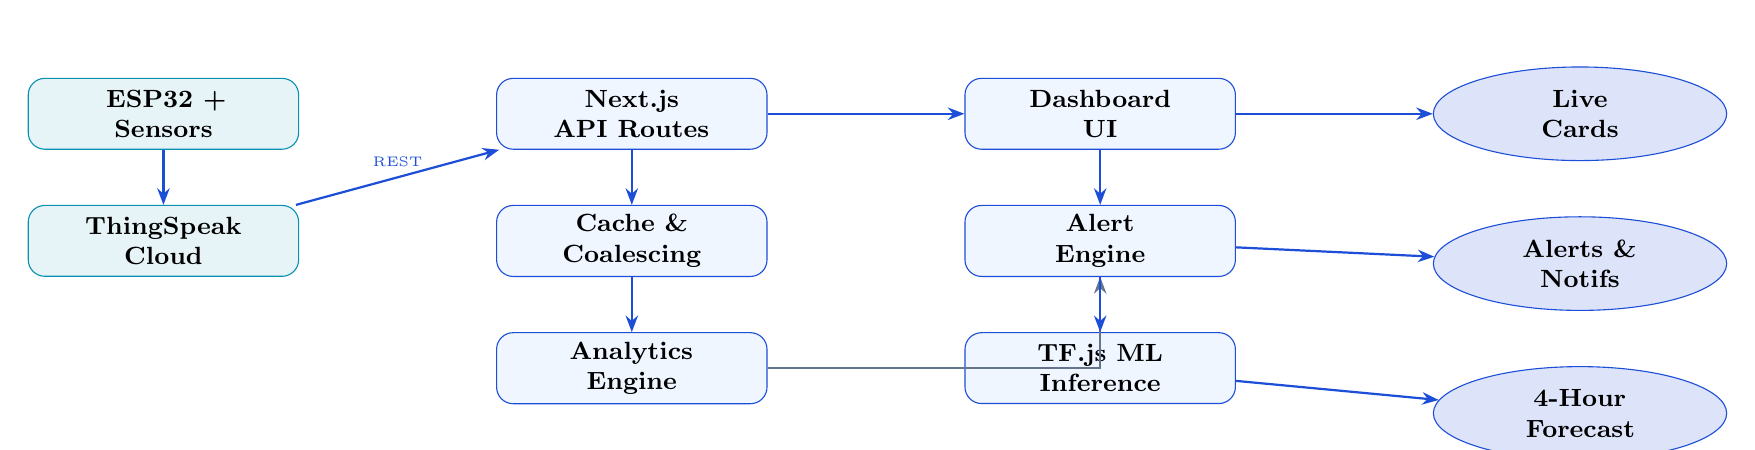
\begin{tikzpicture}[node distance=0.7cm]
  % Column 1: Hardware
  \node[iotbox] (sensor) {ESP32 +\\Sensors};
  \node[iotbox, below=of sensor] (ts) {ThingSpeak\\Cloud};

  % Column 2: Backend
  \node[process, right=2.5cm of sensor] (api) {Next.js\\API Routes};
  \node[process, below=of api] (cache) {Cache \&\\Coalescing};
  \node[process, below=of cache] (analytics) {Analytics\\Engine};

  % Column 3: Frontend
  \node[process, right=2.5cm of api] (dash) {Dashboard\\UI};
  \node[process, below=of dash] (alert) {Alert\\Engine};
  \node[process, below=of alert] (ml) {TF.js ML\\Inference};

  % Column 4: Output
  \node[startend, right=2.5cm of dash] (out1) {Live\\Cards};
  \node[startend, below=of out1] (out2) {Alerts \&\\Notifs};
  \node[startend, below=of out2] (out3) {4-Hour\\Forecast};

  % Arrows col 1
  \draw[arrow] (sensor) -- (ts);
  % Arrows col 1->2
  \draw[arrow] (ts) -- node[above,font=\tiny]{REST} (api);
  % Arrows col 2
  \draw[arrow] (api) -- (cache);
  \draw[arrow] (cache) -- (analytics);
  % Arrows col 2->3
  \draw[arrow] (api) -- (dash);
  \draw[arrowg] (analytics) -| (alert);
  % Arrows col 3
  \draw[arrow] (dash) -- (alert);
  \draw[arrow] (alert) -- (ml);
  % Arrows col 3->4
  \draw[arrow] (dash) -- (out1);
  \draw[arrow] (alert) -- (out2);
  \draw[arrow] (ml) -- (out3);
\end{tikzpicture}%
}
\caption{FloodEye End-to-End Functional Pipeline}
\label{fig:pipeline_overview}
\end{figure}

\section{User Workflow}

A typical user interaction with FloodEye follows this sequence:

\begin{enumerate}[leftmargin=1.5em]
  \item The user navigates to the FloodEye URL (e.g.\ on Vercel) or opens the installed PWA on their device.
  \item The immersive landing page loads with GSAP animations and a background slideshow of flood monitoring imagery.
  \item The user clicks ``Go to Dashboard'' or the direct dashboard link.
  \item The dashboard fetches the latest sensor reading from \texttt{/\allowbreak{}api/\allowbreak{}sensors}. The TelemetryProvider begins polling at the configured refresh interval (default: 15 seconds).
  \item Five sensor cards display live values (Water Level, Temperature, Humidity, Pressure, Altitude) with trend arrows.
  \item Simultaneously, the \texttt{useFloodPrediction} hook loads the TensorFlow.js model from \texttt{/\allowbreak{}public/\allowbreak{}tfjs\_\allowbreak{}model/\allowbreak{}} and, once the model is ready and at least one reading is available (padded with sample data if necessary), runs inference to display the 4-hour water level forecast.
  \item If any sensor reading breaches a configured threshold, an alert card appears in the Alert Panel. Critical alerts trigger a native browser push notification (if permission was granted).
  \item The user can navigate to the \textbf{Analytics} page to view per-channel time-series charts with the time-window selector.
  \item The \textbf{History} page presents a statistical summary table and allows download of sensor logs as CSV or PDF.
  \item The \textbf{Predictions} page provides a detailed ML forecasting panel with risk gauge and feature contributions.
  \item The \textbf{Alerts} page shows the full alert log, filterable by severity.
  \item Admin users can navigate to \textbf{Settings} to adjust alert thresholds, refresh interval, and toggle simulation mode.
\end{enumerate}

\section{Navigation Structure}

FloodEye has two main navigation zones:

\begin{itemize}[leftmargin=1.5em]
  \item \textbf{Landing Zone:} Root route (\texttt{/\allowbreak{}}) — the scrollytelling landing page with navigation bar, hero section, feature showcase, team profiles, and technology section.
  \item \textbf{Dashboard Zone:} All routes under \texttt{/\allowbreak{}dashboard} — protected by a shared layout with a sidebar navigation containing: Dashboard, Analytics, History, Predictions, Alerts, Devices, and Settings.
\end{itemize}

%=============================================================================
% Chapter 4: System Architecture
%=============================================================================
\chapter{System Architecture}

\section{Architectural Overview}

FloodEye follows a three-tier architecture consisting of an IoT hardware layer, a cloud-connected backend layer, and a client-side frontend layer. All tiers are orchestrated through the Next.js full-stack framework, which unifies the backend API routes and the React frontend into a single deployable unit. Figure~\ref{fig:system_arch} illustrates the overall architecture.

\begin{figure}[H]
\centering
\resizebox{\linewidth}{!}{%
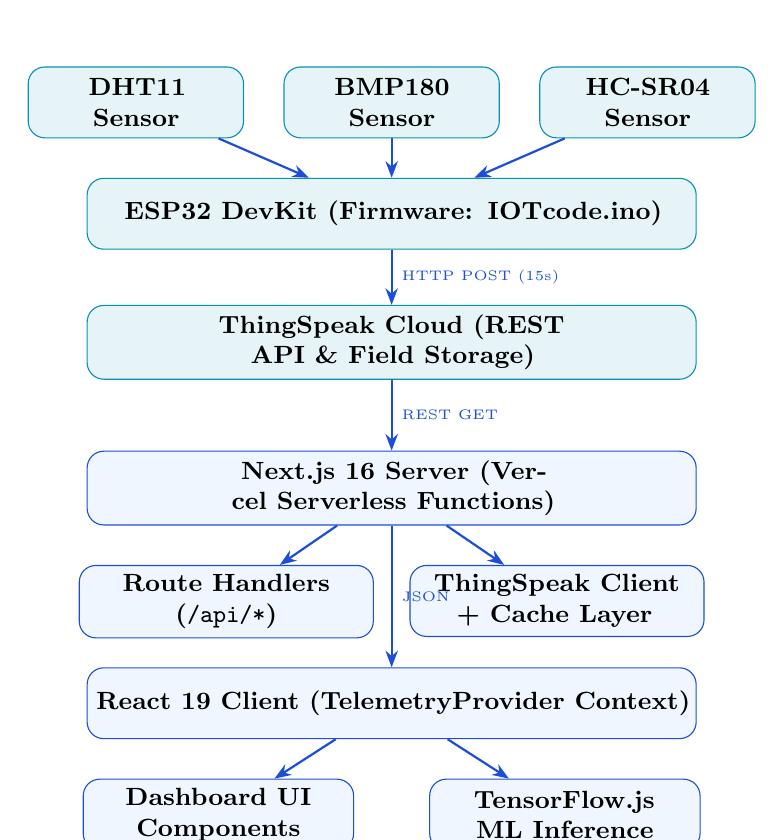
\begin{tikzpicture}[node distance=0.9cm, every node/.style={font=\small}]
  % ── IoT Layer ──
  \node[iotbox, text width=2.5cm] (dht) {DHT11\\Sensor};
  \node[iotbox, text width=2.5cm, right=0.5cm of dht] (bmp) {BMP180\\Sensor};
  \node[iotbox, text width=2.5cm, right=0.5cm of bmp] (hc) {HC-SR04\\Sensor};

  \node[iotbox, text width=7.5cm, below=0.5cm of bmp] (esp) {ESP32 DevKit (Firmware: IOTcode.ino)};

  \node[iotbox, text width=7.5cm, below=0.7cm of esp] (ts) {ThingSpeak Cloud (REST API \& Field Storage)};

  % ── Backend Layer ──
  \node[process, text width=7.5cm, below=0.9cm of ts] (next) {Next.js 16 Server (Vercel Serverless Functions)};
  \node[process, text width=3.5cm, below=0.5cm of next, xshift=-2.1cm] (apiroute) {Route Handlers\\(\texttt{/api/*})};
  \node[process, text width=3.5cm, below=0.5cm of next, xshift=2.1cm] (tscache) {ThingSpeak Client\\+ Cache Layer};

  % ── Frontend Layer ──
  \node[process, text width=7.5cm, below=1.0cm of next, yshift=-0.8cm] (react) {React 19 Client (TelemetryProvider Context)};
  \node[process, text width=3.2cm, below=0.5cm of react, xshift=-2.2cm] (ui) {Dashboard UI\\Components};
  \node[process, text width=3.2cm, below=0.5cm of react, xshift=2.2cm] (tfjs) {TensorFlow.js\\ML Inference};

  % ── Arrows ──
  \draw[arrow] (dht) -- (esp);
  \draw[arrow] (bmp) -- (esp);
  \draw[arrow] (hc) -- (esp);
  \draw[arrow] (esp) -- node[right,font=\tiny]{HTTP POST (15s)} (ts);
  \draw[arrow] (ts) -- node[right,font=\tiny]{REST GET} (next);
  \draw[arrow] (next) -- (apiroute);
  \draw[arrow] (next) -- (tscache);
  \draw[arrow] (next) -- node[right,font=\tiny]{JSON} (react);
  \draw[arrow] (react) -- (ui);
  \draw[arrow] (react) -- (tfjs);
\end{tikzpicture}%
}
\caption{FloodEye Three-Tier System Architecture}
\label{fig:system_arch}
\end{figure}

\section{IoT Hardware Layer}

The hardware layer consists of an ESP32 DevKit microcontroller connected to three sensors:

\begin{itemize}[leftmargin=1.5em]
  \item \textbf{BMP180 (I\textsuperscript{2}C):} Measures atmospheric pressure (hPa) and derives altitude (m). Connected via I\textsuperscript{2}C bus on GPIO 21 (SDA) and GPIO 22 (SCL).
  \item \textbf{DHT11 (Digital):} Measures ambient temperature (°C) and relative humidity (\%). A simple single-wire digital sensor.
  \item \textbf{HC-SR04 (GPIO):} Ultrasonic distance sensor. The distance reading, in centimetres, represents the proximity to the water surface (inversely proportional to water level).
\end{itemize}

The firmware (\texttt{IOTcode/IOTcode.ino}) initialises the BMP180 via the \texttt{Adafruit\_BMP085} library and polls readings in a 2-second loop, printing values to the serial monitor. The full deployment extends this sketch to post field values to ThingSpeak via an HTTP client library.

\section{ThingSpeak Cloud Layer}

ThingSpeak serves as the cloud IoT data platform. The ESP32 uploads to a ThingSpeak channel, whose five fields are mapped as shown in Table~\ref{tab:thingspeak_fields}.

\begin{table}[H]
\centering
\caption{ThingSpeak Channel Field Mapping}
\label{tab:thingspeak_fields}
\begin{tabular}{|c|l|l|}
\hline
\rowcolor{FloodLight}
\textbf{ThingSpeak Field} & \textbf{Sensor} & \textbf{Unit} \\
\hline
Field 1 & Temperature (DHT11) & °C \\
Field 2 & Humidity (DHT11) & \% \\
Field 3 & Atmospheric Pressure (BMP180) & hPa \\
Field 4 & Altitude (BMP180) & m \\
Field 5 & Water Distance (HC-SR04) & cm \\
\hline
\end{tabular}
\end{table}

ThingSpeak imposes a free-tier rate limit of one update per 15 seconds, which aligns with the ESP32 firmware upload interval. The REST API supports both ``last entry'' and ``range'' queries used by the Next.js backend.

\section{Backend Layer}

The backend is implemented as Next.js Route Handlers (the App Router equivalent of API routes). All server logic resides in the \texttt{app/api/} directory. The key components are:

\begin{itemize}[leftmargin=1.5em]
  \item \textbf{\texttt{lib/thingspeak.ts}:} A server-side ThingSpeak client with an in-memory cache and request coalescing. The latest-reading cache has a 14-second TTL (just under the 15-second upload interval); the history cache has a 55-second TTL. Request coalescing prevents cache stampedes when multiple server renders arrive simultaneously.
  \item \textbf{Route Handlers:} \texttt{/api/sensors}, \texttt{/api/history}, \texttt{/api/analytics}, \texttt{/api/environment-score}, \texttt{/api/flood-predict} (placeholder for server-side inference). Each returns a structured JSON response.
  \item \textbf{Incremental Static Revalidation (ISR):} The \texttt{revalidate} export constant on each route sets the Next.js CDN cache TTL (15 s for sensors, 60 s for history/analytics).
\end{itemize}

\section{Frontend Layer}

The frontend is a React 19 application built with Next.js App Router. The central state management mechanism is the \textbf{TelemetryProvider}, a React Context provider that:

\begin{itemize}[leftmargin=1.5em]
  \item Polls \texttt{/api/sensors} at a configurable interval (default 15 s).
  \item Persists the latest reading and history in \texttt{localStorage} for offline resilience.
  \item Evaluates alerts on every new data point using the \texttt{evaluateAlerts()} function.
  \item Exposes telemetry data, history array, alert list, device status, and settings to all child components via the \texttt{useTelemetry()} hook.
\end{itemize}

The ML inference layer runs separately in the \textbf{\texttt{useFloodPrediction}} hook, which loads the TensorFlow.js model from \texttt{/public/tfjs\_model/}, engineers the 11 input features from the history array, and calls \texttt{predictFloodRisk()} to obtain a 4-hour water level forecast.

\section{Data Flow}

The complete data flow from sensor reading to dashboard visualisation is:

\begin{enumerate}[leftmargin=1.5em]
  \item ESP32 reads sensor values and HTTP-POSTs them to ThingSpeak (every 15 s).
  \item ThingSpeak stores the reading in its channel database.
  \item The Next.js server's \texttt{TelemetryProvider} polls \texttt{/api/sensors} (every 15 s).
  \item \texttt{/api/sensors} calls \texttt{getLatestReading()} in \texttt{lib/thingspeak.ts}, which fetches \\ \texttt{https://api.thingspeak.com/channels/\{id\}/feeds/last.json} and parses the five field values into a typed \texttt{TelemetryData} object.
  \item The result is cached for 14 s and returned as JSON to the frontend.
  \item The TelemetryProvider stores the new reading in state and history, evaluates alerts, and persists to \texttt{localStorage}.
  \item All dashboard components subscribed to \texttt{useTelemetry()} re-render with fresh data.
  \item Concurrently, the \texttt{useFloodPrediction} hook detects a new history entry and schedules an ML inference run (debounced by 1 s).
  \item The inference result updates the FloodPredictionCard and FloodPredictionPanel with the new forecast.
\end{enumerate}

\section{Cloud and Deployment Architecture}

FloodEye is deployed on Vercel using its Git-integrated continuous deployment pipeline. Each push to the main branch triggers an automatic build and deployment. Key architectural features of the deployment:

\begin{itemize}[leftmargin=1.5em]
  \item \textbf{Serverless Edge Functions:} Next.js Route Handlers are deployed as Vercel serverless functions, scaling automatically to handle traffic spikes.
  \item \textbf{CDN Caching:} ISR cache headers ensure that the ThingSpeak API is not hammered during high-traffic periods; cached responses are served from Vercel's global CDN edge network.
  \item \textbf{Environment Variables:} ThingSpeak credentials (\texttt{THINGSPEAK\_CHANNEL\_ID}, \texttt{THINGSPEAK\_READ\_API\_KEY}) and the MapTiler key (\texttt{NEXT\_PUBLIC\_MAPTILER\_KEY}) are injected as Vercel environment variables, never exposed in the repository.
  \item \textbf{PWA Service Worker:} The \texttt{next-pwa} package generates a Workbox service worker that caches static assets for offline access.
\end{itemize}

%=============================================================================
% Chapter 5: Technology Stack
%=============================================================================
\chapter{Technology Stack}

This chapter documents every technology used in FloodEye, explaining the purpose of each component and the rationale for its selection.

\section{Frontend Technologies}

\subsection{Next.js 16 (App Router)}
\textbf{Purpose:} Full-stack React framework providing server-side rendering, API routes, file-system-based routing, and seamless Vercel deployment.\\
\textbf{Why chosen:} Next.js App Router colocates server components, client components, and API handlers in a single project. Its ISR (Incremental Static Regeneration) with the \texttt{revalidate} export allows fine-grained cache control per API route without a separate caching layer. The Vercel deployment integration is zero-configuration.\\
\textbf{Version:} 16.2.10

\subsection{React 19}
\textbf{Purpose:} UI component library; the foundation of all dashboard views.\\
\textbf{Why chosen:} React 19 introduces concurrent features and improved suspense semantics. The Context API (\texttt{TelemetryProvider}) serves as lightweight global state management without requiring Redux or Zustand.

\subsection{TypeScript 5}
\textbf{Purpose:} Static typing for all source files (\texttt{.\allowbreak{}ts}, \texttt{.\allowbreak{}tsx}).\\
\textbf{Why chosen:} TypeScript eliminates entire categories of runtime errors in the type-rich data pipeline (ThingSpeak field parsing, TelemetryData objects, alert severity enums). The \texttt{FloodPredictionResult}, \texttt{TelemetryData}, \texttt{DashboardSettings}, and \texttt{Alert} interfaces are all strongly typed.

\subsection{Tailwind CSS v4}
\textbf{Purpose:} Utility-first CSS framework for all component styling.\\
\textbf{Why chosen:} Tailwind v4's JIT (just-in-time) compiler generates minimal CSS bundles. The glassmorphism design language (\texttt{bg-white/\allowbreak{}40 backdrop-blur-xl border-white/\allowbreak{}60}) is cleanly expressed with utility classes without custom CSS files.

\subsection{shadcn/ui}
\textbf{Purpose:} Accessible, unstyled component primitives for buttons, dialogs, and form elements.\\
\textbf{Why chosen:} shadcn/ui components are installed directly into the project source rather than as an opaque dependency, making them fully customisable.

\subsection{Recharts 3}
\textbf{Purpose:} SVG-based charting library for all time-series line charts.\\
\textbf{Why chosen:} Recharts integrates naturally with React's rendering model. It provides \texttt{ResponsiveContainer}, \texttt{LineChart}, \texttt{Tooltip}, and \texttt{CartesianGrid} out-of-the-box, which are sufficient for FloodEye's chart requirements without the configuration overhead of D3.

\subsection{MapLibre GL JS 5 + MapTiler}
\textbf{Purpose:} WebGL-accelerated interactive map rendering.\\
\textbf{Why chosen:} MapLibre GL is an open-source fork of Mapbox GL with no usage-based pricing caps. MapTiler provides high-quality raster and vector tile services compatible with MapLibre's style spec. The \texttt{react-map-gl} wrapper provides React-native integration.

\subsection{Framer Motion 12}
\textbf{Purpose:} Animation library for UI micro-animations, card hover effects, and page transitions.\\
\textbf{Why chosen:} Framer Motion provides a declarative API (\texttt{motion.\allowbreak{}div}, \texttt{AnimatePresence}) that integrates directly with React's component tree.

\subsection{GSAP 3 + @gsap/react}
\textbf{Purpose:} ScrollTrigger-based animations on the landing page.\\
\textbf{Why chosen:} GSAP is the industry standard for high-performance scroll-driven animations. The \texttt{ScrollytellingSections} component uses GSAP's \texttt{fromTo} and \texttt{ScrollTrigger} to choreograph section entrance animations.

\subsection{Lenis 1.3}
\textbf{Purpose:} Smooth, physics-based scroll inertia on the landing page.\\
\textbf{Why chosen:} Lenis provides buttery-smooth native scroll override that pairs naturally with GSAP ScrollTrigger.

\subsection{Lucide React}
\textbf{Purpose:} Icon library providing \texttt{Thermometer}, \texttt{Droplets}, \texttt{Wind}, \texttt{Mountain}, \texttt{Ruler}, \texttt{WifiOff}, \texttt{AlertTriangle}, and other icons used throughout the dashboard.

\subsection{jsPDF + jspdf-autotable}
\textbf{Purpose:} Client-side PDF generation for the sensor history export on the History page.\\
\textbf{Why chosen:} No server is required; the PDF is generated entirely in the browser and downloaded directly.

\section{Machine Learning Technologies}

\subsection{TensorFlow 2 / Keras (Training)}
\textbf{Purpose:} Python deep learning framework used to define, train, and export the flood prediction model.\\
\textbf{Role:} The model is defined in \texttt{Model/\allowbreak{}nb\_\allowbreak{}code.\allowbreak{}py} (extracted from \texttt{FloodMonitoring.\allowbreak{}ipynb}). Training runs in Google Colab with GPU acceleration.

\subsection{TensorFlow.js 4.22 (Inference)}
\textbf{Purpose:} JavaScript port of TensorFlow; runs the trained model in the browser using WebGL acceleration.\\
\textbf{Why chosen:} Client-side inference eliminates the need for a dedicated ML serving infrastructure. The model runs on the user's device with no server cost for inference.\\
\textbf{Integration:} The custom \texttt{AttentionLayer} is reimplemented in TypeScript and registered with \texttt{tf.\allowbreak{}serialization.\allowbreak{}registerClass()} before model loading.

\subsection{scikit-learn StandardScaler}
\textbf{Purpose:} Feature normalisation during training.\\
\textbf{Role:} Scaler parameters (mean and scale vectors) are exported to \texttt{scalers.\allowbreak{}json} and loaded by the browser at inference time to apply the same normalisation.

\subsection{TensorFlow.js Converter}
\textbf{Purpose:} Converts the trained Keras \texttt{.\allowbreak{}h5} model to TensorFlow.js LayersModel format (\texttt{model.\allowbreak{}json} + \texttt{group1-shard1of1.\allowbreak{}bin}).

\section{Backend Technologies}

\subsection{Next.js Route Handlers}
\textbf{Purpose:} Serverless API endpoints at \texttt{app/\allowbreak{}api/\allowbreak{}*/\allowbreak{}route.\allowbreak{}ts}.

\subsection{ThingSpeak REST API}
\textbf{Purpose:} IoT cloud data platform; stores and serves field-mapped sensor readings.

\section{IoT Technologies}

\subsection{ESP32 DevKit}
\textbf{Purpose:} Main microcontroller; reads sensors and uploads data to ThingSpeak via Wi-Fi.\\
\textbf{Framework:} Arduino (C++ sketch: \texttt{IOTcode/\allowbreak{}IOTcode.\allowbreak{}ino}).

\subsection{Adafruit BMP085 Library}
\textbf{Purpose:} Arduino driver for the BMP180 pressure and temperature sensor.

\subsection{DHT Sensor Library}
\textbf{Purpose:} Arduino driver for the DHT11 temperature and humidity sensor.

\section{Development Tools}

\begin{table}[H]
\centering
\caption{Development Tools and Versions}
\begin{tabularx}{\linewidth}{|l|l|X|}
\hline
\rowcolor{FloodLight}
\textbf{Tool} & \textbf{Version} & \textbf{Purpose} \\
\hline
Node.js & v20.x & JavaScript runtime \\
npm & v10.x & Package manager \\
TypeScript & 5.x & Static type checking \\
ESLint & 9.x & Code quality linting \\
PostCSS & 4.x & Tailwind CSS processing \\
Google Colab & --- & GPU-accelerated ML training environment \\
Arduino IDE & --- & ESP32 firmware development and flashing \\
\hline
\end{tabularx}
\end{table}

\section{Hosting and Infrastructure}

\begin{table}[H]
\centering
\caption{Hosting and Infrastructure}
\begin{tabularx}{\linewidth}{|l|X|}
\hline
\rowcolor{FloodLight}
\textbf{Service} & \textbf{Role} \\
\hline
Vercel & Next.js application hosting; serverless functions; CDN; CI/CD pipeline \\
ThingSpeak & IoT cloud data storage and REST API \\
MapTiler & Vector tile service for MapLibre GL interactive map \\
\hline
\end{tabularx}
\end{table}

%=============================================================================
% Chapter 6: Frontend Implementation
%=============================================================================
\chapter{Frontend Implementation}

The FloodEye frontend is a Next.js 16 App Router application. All pages live under either the root \texttt{/} (landing) or the nested \texttt{/dashboard/} route group. This chapter describes each page in detail.

\section{Landing Page (\texttt{app/page.tsx})}

\subsection{Purpose}
The landing page serves as the public-facing introduction to FloodEye. It is designed to be visually striking and informative, communicating the project's purpose to new visitors before they enter the monitoring dashboard.

\subsection{Components}
\begin{itemize}[leftmargin=1.5em]
  \item \textbf{LandingNav:} Fixed top navigation bar with logo, navigation links, and a ``Go to Dashboard'' call-to-action button. Includes blur-glass styling.
  \item \textbf{BackgroundSlideshow:} An auto-advancing slideshow of flood monitoring imagery rendered as a full-viewport background layer.
  \item \textbf{ScrollytellingSections:} The primary content component. Uses GSAP ScrollTrigger to animate content sections as the user scrolls: Hero, Problem Statement, Features Showcase, Technology Stack, Team Profiles (with individual member photos from \texttt{/public/}), and a call-to-action.
  \item \textbf{AssamNodeMap:} A landing-page specific map component showing the geographic coverage area of the monitoring network in Assam.
  \item \textbf{PWAInstallPrompt:} A floating prompt that appears when the browser's beforeinstallprompt event fires, inviting the user to install the PWA.
\end{itemize}

\subsection{Key Features}
\begin{itemize}[leftmargin=1.5em]
  \item Lenis smooth scroll integration for physics-based scroll inertia.
  \item GSAP \texttt{fromTo} and \texttt{ScrollTrigger} animations for each section entrance.
  \item Fully responsive layout adapting from mobile through desktop breakpoints.
  \item Team member profile cards with photos from the public directory.
\end{itemize}

\section{Dashboard Home (\texttt{app/dashboard/page.tsx})}

\subsection{Purpose}
The main dashboard provides a comprehensive real-time overview of all sensor readings, device status, live charts, alerts, and the flood risk prediction in a single scrollable view.

\subsection{Layout Structure}

The dashboard is organised in four rows:

\begin{enumerate}[leftmargin=1.5em]
  \item \textbf{Row 1:} Five sensor cards (Temperature, Humidity, Pressure, Altitude, Water Level) in a responsive grid (1 col on mobile \textrightarrow{} 5 cols on XL screens).
  \item \textbf{Row 2:} A 2:1 grid containing the Water Level Trend chart (left, spanning 2 columns) and a right column with ComfortScoreCard, FloodPredictionCard, and DeviceStatusCard stacked vertically.
  \item \textbf{Row 3:} The AlertPanel spanning the full width.
  \item \textbf{Row 4:} The interactive sensor location map (MapLibre GL, loaded dynamically with SSR disabled).
\end{enumerate}

\subsection{Sensor Cards (SensorCard Component)}

Each SensorCard renders:
\begin{itemize}[leftmargin=1.5em]
  \item Current reading with unit.
  \item Trend arrow icon (up / down / stable) calculated by comparing the current reading against the previous one.
  \item Delta value showing the numeric change from the previous reading.
  \item A sparkline mini-chart rendered using the \texttt{historyData} prop.
  \item A status badge (normal / warning / critical) with colour coding.
  \item Offline-state: Cards are labelled ``(Cached)'' when the device is offline.
\end{itemize}

Alert thresholds per card:
\begin{itemize}[leftmargin=1.5em]
  \item Temperature $>$ 35°C: warning status.
  \item Humidity $>$ 80\%: warning status.
  \item Water Level $<$ 20 cm: critical; $<$ 40 cm: warning.
\end{itemize}

\subsection{Water Level Trend Chart}
An interactive Recharts \texttt{CustomLineChart} displays the last N data points of water level (cm) vs.\ time. A ``Live'' or ``Cached'' pill badge indicates the current data freshness.

\subsection{Comfort Score Card}
Calculates and displays the Environmental Comfort Score as a percentage derived from temperature and humidity. Score ranges map to qualitative labels (Excellent / Good / Moderate / Poor).

\subsection{Flood Prediction Card}
A compact summary of the ML prediction result: predicted water level in 4 hours, risk level badge (Low / Moderate / High / Critical), and flood probability percentage.

\subsection{Device Status Card}
Displays ESP32 online/offline status, ThingSpeak connection status, and last upload time derived from the \texttt{DeviceStatus} object.

\subsection{Alert Panel}
The AlertPanel component renders a horizontally scrollable list of active alerts, with severity-coded colour bands. It links to the full Alerts page.

\subsection{Offline Behaviour}
When the ESP32 is unreachable:
\begin{itemize}[leftmargin=1.5em]
  \item An orange \textbf{OfflineBanner} is shown at the top with the time of the last live reading.
  \item Sensor cards show ``(Cached)'' labels.
  \item The Live badge on the chart changes to ``Cached''.
  \item A \textbf{NoDataState} component replaces the dashboard if no cached data exists at all.
\end{itemize}

\section{Analytics Page (\texttt{app/dashboard/analytics/page.tsx})}

\subsection{Purpose}
Provides individual time-series charts for all five sensor channels, each rendered in its own card.

\subsection{Components}
\begin{itemize}[leftmargin=1.5em]
  \item \textbf{TimeFilter:} A pill-tab selector for 1h, 6h, 24h, 7d, 30d windows. Selecting a window triggers a new \texttt{/api/history?range=\{window\}} request.
  \item \textbf{Five CustomLineChart cards:} Temperature (°C), Humidity (\%), Atmospheric Pressure (hPa), Altitude (m), Water Level (cm). The Water Level card uses a dark gradient background to visually distinguish it as the primary safety metric.
  \item The Pressure chart spans two columns (\texttt{lg:col-span-2}) as a wide chart for better readability.
\end{itemize}

\section{History Page (\texttt{app/dashboard/history/page.tsx})}

\subsection{Purpose}
Displays statistical summaries of sensor history and provides data export functionality.

\subsection{Components}
\begin{itemize}[leftmargin=1.5em]
  \item \textbf{StatCard grid:} Six cards showing average, min, and max for temperature, humidity, and water level across the current history window.
  \item \textbf{Data table:} A scrollable table of the last 100 readings with columns: Time, Temperature, Humidity, Pressure, Altitude, Water Level.
  \item \textbf{Export buttons:}
    \begin{itemize}
      \item \textbf{CSV Export:} Generates a Blob from the history array and downloads it as \texttt{floodeye\_logs\_\{date\}.csv}.
      \item \textbf{PDF Export:} Uses jsPDF + jspdf-autotable to generate a formatted PDF with the FloodEye header and a data table.
    \end{itemize}
\end{itemize}

\section{Predictions Page (\texttt{app/dashboard/predictions/page.tsx})}

\subsection{Purpose}
A dedicated full-page view of the ML flood forecasting results with admin diagnostic tools.

\subsection{Components}
\begin{itemize}[leftmargin=1.5em]
  \item \textbf{FloodPredictionPanel:} A large card displaying the predicted water level, a circular risk gauge, flood probability bar, confidence score, feature contributions list (Water Level, Temperature, Humidity, Pressure), and a timestamp of the last inference.
  \item \textbf{Admin Diagnostics (admin role only):}
    \begin{itemize}
      \item Model Architecture card: Type (CNN-BiLSTM-Att), Input Shape [48, 11], Output (4hr Forecast), MAE (Train: 3.42 cm).
      \item Inference Engine card: Provider (TensorFlow.js/WebGL), live status (COMPUTING/READY), last run timestamp.
      \item Settings CTA card: Links to the Settings page.
    \end{itemize}
\end{itemize}

\section{Alerts Page (\texttt{app/dashboard/alerts/page.tsx})}

\subsection{Purpose}
The full alert log with severity filtering and per-alert dismissal.

\subsection{Components}
\begin{itemize}[leftmargin=1.5em]
  \item Summary badges showing counts of Critical, Warning, and Info alerts.
  \item \textbf{AlertCard:} Each alert card displays: severity icon, type label, severity badge, timestamp (relative, e.g.\ ``3m ago''), message text, and a dismiss button.
  \item Alerts are ordered critical-first, then warning, then info.
  \item ``Clear All'' button clears the log and resets all alert cooldown timers.
\end{itemize}

\textbf{Alert types implemented:}
\begin{itemize}[leftmargin=1.5em]
  \item HIGH\_TEMPERATURE, HIGH\_HUMIDITY, RAPID\_PRESSURE\_CHANGE
  \item HIGH\_WATER\_LEVEL, RAPID\_WATER\_RISE, OBJECT\_TOO\_CLOSE, SENSOR\_OFFLINE
\end{itemize}

\section{Settings Page (\texttt{app/dashboard/settings/page.tsx})}

\subsection{Purpose}
Allows admin users to configure alert thresholds, refresh interval, and simulation mode.

\subsection{Access Control}
The Settings page checks \texttt{userRole === "admin"} from the TelemetryProvider context. Non-admin users see an access-restricted screen with a ShieldAlert icon.

\subsection{Settings Sections}
\begin{itemize}[leftmargin=1.5em]
  \item \textbf{Connection Settings:} Refresh interval selector (5s, 15s, 30s, 60s). Simulation mode toggle (uses synthetic data instead of live ThingSpeak readings).
  \item \textbf{Alert Thresholds:} Input fields for Temperature threshold (°C), Humidity threshold (\%), Water Level threshold (cm), Pressure threshold (hPa).
  \item \textbf{Save:} Persists settings to the TelemetryProvider context (in-memory; not yet persisted to a database in the current implementation).
\end{itemize}

\section{Devices Page (\texttt{app/dashboard/devices/})}

The Devices section provides device management views showing registered ESP32 nodes and their connection status. In the current implementation, this page displays the status of the single configured ThingSpeak channel.

\section{Responsive Design}

All dashboard pages are fully responsive using Tailwind CSS breakpoint utilities:
\begin{itemize}[leftmargin=1.5em]
  \item \textbf{Mobile (default):} Single column layout; cards stack vertically.
  \item \textbf{Tablet (\texttt{sm:}):} Sensor cards 2-column grid.
  \item \textbf{Laptop (\texttt{lg:}):} 3-column grid for sensor cards; 3:1 chart+sidebar split.
  \item \textbf{Desktop (\texttt{xl:}):} 5-column sensor card grid; full analytics 2-column layout.
\end{itemize}

%=============================================================================
% Chapter 7: Application Navigation
%=============================================================================
\chapter{Application Navigation}

\section{Navigation Architecture}

FloodEye uses Next.js App Router's file-system-based routing. The application has two primary zones: the public Landing Zone and the authenticated Dashboard Zone. The dashboard zone uses a shared layout (\texttt{app/\allowbreak{}dashboard/\allowbreak{}layout.\allowbreak{}tsx}) that renders the sidebar navigation on every dashboard page.

\section{Navigation Flow Diagram}

Figure~\ref{fig:nav_flow} illustrates the complete navigation flow of the application.

\begin{figure}[H]
\centering
\resizebox{\linewidth}{!}{%
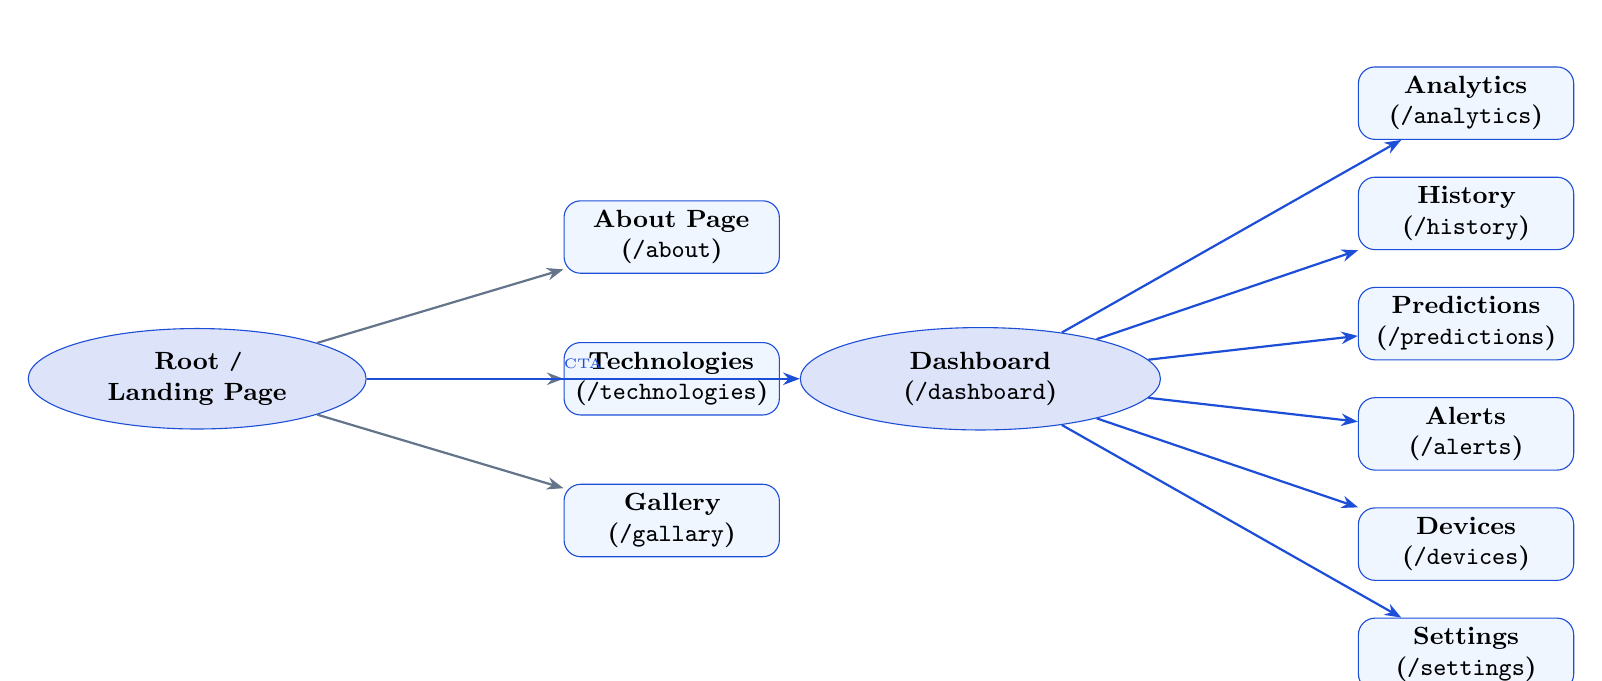
\begin{tikzpicture}[node distance=0.7cm, every node/.style={font=\footnotesize}]
  % Landing
  \node[startend, text width=2.8cm] (root) {Root \texttt{/\allowbreak{}}\\Landing Page};

  % Landing sub-pages
  \node[process, text width=2.5cm, right=2.5cm of root, yshift=1.8cm] (about) {About Page\\(\texttt{/\allowbreak{}about})};
  \node[process, text width=2.5cm, right=2.5cm of root, yshift=0.0cm] (tech) {Technologies\\(\texttt{/\allowbreak{}technologies})};
  \node[process, text width=2.5cm, right=2.5cm of root, yshift=-1.8cm] (gallery) {Gallery\\(\texttt{/\allowbreak{}gallary})};

  % Dashboard entry
  \node[startend, text width=3cm, right=5.5cm of root] (dash) {Dashboard\\(\texttt{/\allowbreak{}dashboard})};

  % Dashboard pages
  \node[process, text width=2.5cm, right=2.5cm of dash, yshift=3.5cm] (analytics) {Analytics\\(\texttt{/\allowbreak{}analytics})};
  \node[process, text width=2.5cm, right=2.5cm of dash, yshift=2.1cm] (history) {History\\(\texttt{/\allowbreak{}history})};
  \node[process, text width=2.5cm, right=2.5cm of dash, yshift=0.7cm] (predict) {Predictions\\(\texttt{/\allowbreak{}predictions})};
  \node[process, text width=2.5cm, right=2.5cm of dash, yshift=-0.7cm] (alerts) {Alerts\\(\texttt{/\allowbreak{}alerts})};
  \node[process, text width=2.5cm, right=2.5cm of dash, yshift=-2.1cm] (devices) {Devices\\(\texttt{/\allowbreak{}devices})};
  \node[process, text width=2.5cm, right=2.5cm of dash, yshift=-3.5cm] (settings) {Settings\\(\texttt{/\allowbreak{}settings})};

  % Arrows from root
  \draw[arrowg] (root) -- (about);
  \draw[arrowg] (root) -- (tech);
  \draw[arrowg] (root) -- (gallery);
  \draw[arrow] (root) -- node[above,font=\tiny]{CTA} (dash);

  % Arrows from dashboard
  \draw[arrow] (dash) -- (analytics);
  \draw[arrow] (dash) -- (history);
  \draw[arrow] (dash) -- (predict);
  \draw[arrow] (dash) -- (alerts);
  \draw[arrow] (dash) -- (devices);
  \draw[arrow] (dash) -- (settings);
\end{tikzpicture}%
}
\caption{FloodEye Complete Navigation Flow}
\label{fig:nav_flow}
\end{figure}

\section{Landing Zone Pages}

\begin{table}[H]
\centering
\caption{Landing Zone Pages}
\begin{tabularx}{\linewidth}{|l|l|X|}
\hline
\rowcolor{FloodLight}
\textbf{Route} & \textbf{Page} & \textbf{Purpose} \\
\hline
\texttt{/\allowbreak{}} & Landing Page & Scrollytelling intro with GSAP animations, feature showcase, team section \\
\hline
\texttt{/\allowbreak{}about} & About & Project background, team details, internship context \\
\hline
\texttt{/\allowbreak{}technologies} & Technologies & Technology stack showcase with animated cards \\
\hline
\texttt{/\allowbreak{}gallary} & Gallery & Project photo gallery and hardware demonstration images \\
\hline
\end{tabularx}
\end{table}

\section{Dashboard Zone Layout}

The dashboard zone uses a shared \texttt{layout.\allowbreak{}tsx} that wraps all \texttt{/\allowbreak{}dashboard/\allowbreak{}*} pages. This layout renders:

\begin{itemize}[leftmargin=1.5em]
  \item \textbf{Sidebar Navigation:} A fixed left sidebar containing:
    \begin{itemize}
      \item FloodEye logo and version.
      \item Navigation links: Dashboard, Analytics, History, Predictions, Alerts, Devices, Settings.
      \item User role indicator (Admin / User) and username display.
      \item Alert bell icon with unread count badge.
    \end{itemize}
  \item \textbf{Top Header Bar:} Displays the current page title, date/time, connection status indicator, and the PWA install button.
  \item \textbf{Main Content Area:} The \texttt{\{children\}} slot where each page renders.
  \item \textbf{TelemetryProvider:} The layout wraps all content in the TelemetryProvider context so every dashboard page has access to live sensor data.
\end{itemize}

\section{Dashboard Pages}

\begin{table}[H]
\centering
\caption{Dashboard Zone Pages and Features}
\begin{tabularx}{\linewidth}{|l|X|}
\hline
\rowcolor{FloodLight}
\textbf{Route} & \textbf{Features} \\
\hline
\texttt{/\allowbreak{}dashboard} & Live sensor cards, water level chart, comfort score, flood prediction card, alert panel, device map \\
\hline
\texttt{/\allowbreak{}dashboard/\allowbreak{}analytics} & Five individual time-series charts, time window selector (1h–30d) \\
\hline
\texttt{/\allowbreak{}dashboard/\allowbreak{}history} & Statistical summary cards, reading table, CSV export, PDF export \\
\hline
\texttt{/\allowbreak{}dashboard/\allowbreak{}predictions} & ML prediction panel, risk gauge, feature contributions, admin diagnostics \\
\hline
\texttt{/\allowbreak{}dashboard/\allowbreak{}alerts} & Full alert log, severity badges, dismiss and clear functionality \\
\hline
\texttt{/\allowbreak{}dashboard/\allowbreak{}devices} & Device registration and status (single-channel in current implementation) \\
\hline
\texttt{/\allowbreak{}dashboard/\allowbreak{}settings} & Threshold configuration, refresh interval, simulation toggle (admin only) \\
\hline
\end{tabularx}
\end{table}

\section{Authentication Routes}

The \texttt{app/\allowbreak{}(auth)/\allowbreak{}} route group contains structural placeholder pages for a future authentication system. In the current implementation, user role is stored in \texttt{localStorage} (key: \texttt{floodeye\_\allowbreak{}session}) and toggled through the Settings page, rather than through a proper login/password flow. This is noted as a known limitation and future enhancement.

\section{PWA Navigation}

When FloodEye is installed as a PWA:
\begin{itemize}[leftmargin=1.5em]
  \item The app opens in a standalone browser window (without browser chrome) displaying the dashboard home.
  \item The service worker (\texttt{public/\allowbreak{}sw.\allowbreak{}js}) caches static assets and serves the last known dashboard state offline.
  \item Native back/forward navigation works as in a native app.
  \item The \texttt{PWAInstallButton} in the top header bar triggers the native install prompt when the PWA is not yet installed.
\end{itemize}

%=============================================================================
% Chapter 8: Backend Implementation
%=============================================================================
\chapter{Backend Implementation}

\section{Overview}

The FloodEye backend is implemented using Next.js App Router Route Handlers, which run as serverless functions on Vercel. There is no separate Express.js or FastAPI server. All backend logic is colocated with the frontend in the single Next.js project.

\section{Folder Structure}

\begin{lstlisting}[language={},caption={Backend-relevant directory structure},label={lst:folder_structure}]
app/
  api/
    sensors/          route.ts   -- GET /api/sensors
    history/          route.ts   -- GET /api/history
    analytics/        route.ts   -- GET /api/analytics
    environment-score/ route.ts  -- GET /api/environment-score
    flood-predict/    route.ts   -- POST /api/flood-predict
lib/
  thingspeak.ts       -- ThingSpeak client + cache
  flood-model.ts      -- TF.js model loader + inference
  utils.ts            -- cn() utility
  actions/            -- Next.js Server Actions (if any)
hooks/
  useFloodPrediction.ts  -- Client-side ML hook
  useNativeNotification.ts
  use-outside-click.ts
components/
  providers/
    TelemetryProvider.tsx  -- Central data/state provider
\end{lstlisting}

\section{ThingSpeak Client (\texttt{lib/thingspeak.ts})}

The ThingSpeak client is the core of the backend data layer. It encapsulates all communication with the ThingSpeak REST API and implements a sophisticated caching strategy to minimise external API calls.

\subsection{Field Parsing}

The \texttt{feedToTelemetry()} function maps ThingSpeak feed fields to the \texttt{TelemetryData} type:

\begin{lstlisting}[language=TypeScript,caption={ThingSpeak field-to-telemetry mapping}]
function feedToTelemetry(feed: ThingSpeakFeed): TelemetryData {
  return {
    temperature: parseField(feed.field1),      // DHT11 temp (deg C)
    humidity:    parseField(feed.field2),      // DHT11 humidity (%)
    pressure:    parseField(feed.field3, 1013.25), // BMP180 (hPa)
    altitude:    parseField(feed.field4),      // BMP180 altitude (m)
    distance:    parseField(feed.field5),      // HC-SR04 distance (cm)
    timestamp:   feed.created_at,
  };
}
\end{lstlisting}

\subsection{Caching and Request Coalescing}

The cache is implemented using a global singleton pattern (\texttt{globalThis.\_\_thingspeakCache}) to persist across serverless function invocations within the same Node.js instance:

\begin{itemize}[leftmargin=1.5em]
  \item \textbf{Latest cache TTL:} 14,000 ms (14 s), just under the 15-second ESP32 upload interval.
  \item \textbf{History cache TTL:} 55,000 ms (55 s), with separate cache slots per query key (range string).
  \item \textbf{Request coalescing:} If a fetch is already in-flight, subsequent callers await the same Promise rather than firing additional parallel requests to ThingSpeak.
  \item \textbf{Stale-while-revalidate:} If a stale (expired) entry exists, it is returned immediately while a background refetch is initiated, preventing blocking.
\end{itemize}

\subsection{Device Online Detection}

The \texttt{deriveDeviceStatus()} function checks whether the ESP32 is online by comparing the ThingSpeak \texttt{created\_at} timestamp against the current time. If the last upload was more than 60 seconds ago, \texttt{esp32Online} is set to \texttt{false}.

\section{API Route Handlers}

\subsection{\texttt{GET /api/sensors}}

Returns the single latest sensor reading as a \texttt{\{data, deviceStatus\}} JSON object. Uses a 15-second ISR revalidation window (\texttt{export const revalidate = 15}).

\subsection{\texttt{GET /api/history?range=\{range\}}}

Returns historical sensor readings mapped from ThingSpeak feeds. The \texttt{rangeToQuery()} function maps time range strings to ThingSpeak query parameters:

\begin{lstlisting}[language=TypeScript,caption={History range-to-query mapping}]
case "1h":  return { results: 240 };   // 240 * 15s = 1 hour
case "6h":  return { results: 1440 };
case "24h": return { results: 5760 };  // ThingSpeak max = 8000
case "7d":  return { start: ..., end: ... };  // date range
case "30d": return { start: ..., end: ... };
\end{lstlisting}

For ranges $>$ 24h, explicit date ranges are used to avoid the 8000-entry cap limiting the effective window to ~33 hours.

\subsection{\texttt{GET /api/analytics?range=\{range\}}}

Fetches history feeds and computes per-sensor statistics. The \texttt{computeStats()} function calculates:
\begin{itemize}[leftmargin=1.5em]
  \item \textbf{avg}, \textbf{min}, \textbf{max}: Standard descriptive statistics over all readings in the window.
  \item \textbf{trend}: Compares the average of the last 10\% of readings against the first 10\% to classify as ``up'', ``down'', or ``stable'' (threshold: $\pm 0.5$ units).
\end{itemize}

Returns: \texttt{\{range, count, analytics: \{temperature, humidity, pressure, altitude, distance\}\}}.

\subsection{\texttt{GET /api/environment-score}}

Fetches the latest reading and computes the Environmental Comfort Score from temperature and humidity using a weighted formula. Returns \texttt{\{score, status\}}.

\subsection{\texttt{POST /api/flood-predict}}

A structural placeholder for future server-side TensorFlow.js Node inference. In the current implementation it validates the request body (must contain a \texttt{history} array of at least 48 entries) and returns HTTP 501 (Not Implemented) with a message directing callers to use the client-side \texttt{lib/flood-model.ts} inference path.

\section{TelemetryProvider (\texttt{components/providers/TelemetryProvider.tsx})}

The TelemetryProvider is the most complex component in the codebase at 566 lines. It serves as the central state management layer for the entire dashboard.

\subsection{State Variables}

\begin{table}[H]
\centering
\caption{TelemetryProvider State Variables}
\begin{tabularx}{\linewidth}{|l|l|X|}
\hline
\rowcolor{FloodLight}
\textbf{Variable} & \textbf{Type} & \textbf{Description} \\
\hline
data & TelemetryData | null & Current (latest) reading \\
history & TelemetryData[] & Rolling history array \\
deviceStatus & DeviceStatus | null & ESP32 and ThingSpeak connection state \\
alerts & Alert[] & Active alert list (max 20) \\
settings & DashboardSettings & Configurable thresholds and refresh interval \\
isLoading & boolean & True during first fetch \\
isOffline & boolean & True when ESP32 is not reachable \\
isStale & boolean & True when offline but cached data exists \\
lastSeenAt & string | null & ISO timestamp of last live reading \\
unreadCount & number & Count of unread alerts \\
isSimulating & boolean & Simulation mode toggle \\
userRole & "admin" | "user" & Current user role \\
userName & string | null & Display name \\
\hline
\end{tabularx}
\end{table}

\subsection{Alert Engine}

The \texttt{evaluateAlerts()} function is called on every new data point and returns an array of alert payloads based on threshold comparisons. Alert logic covers:

\begin{itemize}[leftmargin=1.5em]
  \item \textbf{RAPID\_WATER\_RISE:} Water rose $\geq$ 5 cm since the previous reading (critical).
  \item \textbf{HIGH\_WATER\_LEVEL:} Distance below \texttt{distanceThreshold}; sub-60\% is critical.
  \item \textbf{RAPID\_PRESSURE\_CHANGE:} Pressure below threshold with $>$ 2 hPa drop, or $<$ 998 hPa.
  \item \textbf{HIGH\_TEMPERATURE:} Temperature $>$ \texttt{tempThreshold} + 1°C margin.
  \item \textbf{HIGH\_HUMIDITY:} Humidity $>$ \texttt{humidityThreshold} + 2\% margin.
\end{itemize}

Per-type cooldowns prevent alert spam:

\begin{table}[H]
\centering
\caption{Alert Cooldown Configuration}
\begin{tabular}{|l|r|}
\hline
\rowcolor{FloodLight}
\textbf{Alert Type} & \textbf{Cooldown} \\
\hline
HIGH\_TEMPERATURE & 5 min \\
HIGH\_HUMIDITY & 5 min \\
RAPID\_PRESSURE\_CHANGE & 3 min \\
HIGH\_WATER\_LEVEL & 2 min \\
RAPID\_WATER\_RISE & 1 min \\
OBJECT\_TOO\_CLOSE & 2 min \\
SENSOR\_OFFLINE & 10 min \\
\hline
\end{tabular}
\end{table}

\subsection{Local Storage Persistence}

Four localStorage keys provide offline resilience:
\begin{itemize}[leftmargin=1.5em]
  \item \texttt{ecosense:lastData} — latest telemetry reading.
  \item \texttt{ecosense:lastHistory} — last known history array.
  \item \texttt{ecosense:lastStatus} — last device status.
  \item \texttt{ecosense:lastSeenAt} — ISO timestamp of last live contact.
\end{itemize}

On mount, if \texttt{/api/sensors} returns null (offline), the provider hydrates from localStorage so the dashboard has data to show immediately.

\section{Request–Response Lifecycle}

\begin{enumerate}[leftmargin=1.5em]
  \item Browser mounts the dashboard; \texttt{TelemetryProvider} calls \texttt{/api/sensors}.
  \item Next.js server handler calls \texttt{getLatestReading()} in \texttt{lib/thingspeak.ts}.
  \item Cache is checked: if fresh (age $<$ 14s), cached result is returned immediately.
  \item If stale or empty: ThingSpeak REST endpoint is fetched; result is parsed, stored in cache, and returned.
  \item Response travels back to the TelemetryProvider as a typed \texttt{TelemetryData} object.
  \item Provider updates React state, persists to localStorage, evaluates alerts.
  \item All subscribed components re-render. Total round-trip: $<$ 200 ms when cached.
\end{enumerate}

%=============================================================================
% Chapter 9: Database Design
%=============================================================================
\chapter{Database Design}

\section{Data Storage Strategy}

FloodEye employs a distributed data storage strategy consisting of three complementary layers rather than a single monolithic database:

\begin{enumerate}[leftmargin=1.5em]
  \item \textbf{ThingSpeak Cloud Storage:} The primary time-series store for all sensor readings. ThingSpeak acts as the IoT backend database, storing every field-mapped reading uploaded by the ESP32 with a UTC timestamp and an auto-incrementing \texttt{entry\_\allowbreak{}id}.
  \item \textbf{Browser localStorage:} A client-side persistence layer that stores the last known sensor reading, history array, device status, and last-seen timestamp. This enables offline resilience when the ESP32 or ThingSpeak is unreachable.
  \item \textbf{In-Memory Server Cache:} The Next.js server maintains an in-process cache (using \texttt{globalThis.\allowbreak{}\_\allowbreak{}\_\allowbreak{}thingspeakCache}) that prevents repeated API calls to ThingSpeak within the cache TTL window.
\end{enumerate}

\textit{Note: The project documentation (\texttt{TIHDash.\allowbreak{}md}) references a Neon PostgreSQL database for storing users, devices, alert history, and settings. In the current implementation, this database layer is not active. All session data, settings, and alerts are managed in-memory/localStorage only. A Neon PostgreSQL integration is identified as a future enhancement.}

\section{ThingSpeak Data Model}

\subsection{Channel Structure}

ThingSpeak organises data into channels, each containing up to eight fields. FloodEye uses five fields:

\begin{table}[H]
\centering
\caption{ThingSpeak Data Schema}
\begin{tabularx}{\linewidth}{|l|l|l|X|}
\hline
\rowcolor{FloodLight}
\textbf{Field} & \textbf{Name} & \textbf{Type} & \textbf{Description} \\
\hline
\texttt{field1} & temperature & FLOAT & DHT11 temperature reading in °C \\
\texttt{field2} & humidity & FLOAT & DHT11 relative humidity in \% \\
\texttt{field3} & pressure & FLOAT & BMP180 atmospheric pressure in hPa \\
\texttt{field4} & altitude & FLOAT & BMP180 derived altitude in metres \\
\texttt{field5} & distance & FLOAT & HC-SR04 distance to water surface in cm \\
\texttt{created\_\allowbreak{}at} & timestamp & DATETIME & UTC timestamp of the upload \\
\texttt{entry\_\allowbreak{}id} & id & INTEGER & Auto-increment entry identifier \\
\hline
\end{tabularx}
\end{table}

\subsection{Data Access Patterns}

Two primary query patterns are used:

\begin{enumerate}[leftmargin=1.5em]
  \item \textbf{Latest Entry:} \texttt{GET /\allowbreak{}channels/\allowbreak{}\{id\}/feeds/last.json?api\_key=\{key\}} --- Returns a single JSON object (the most recent feed entry). Used by \texttt{/\allowbreak{}api/\allowbreak{}sensors}.
  \item \textbf{Historical Range:}
    \begin{itemize}
      \item By count: \texttt{GET /\allowbreak{}channels/\allowbreak{}\{id\}/feeds.json?results=N\&api\_key=\{key\}} --- Returns the last N entries (max 8000 per call). Used for ranges $\leq$ 24h.
      \item By date range: \texttt{GET /\allowbreak{}channels/\allowbreak{}\{id\}/feeds.json?start=\{dt\}\&end=\{dt\}\&api\_key=\{key\}} --- Returns all entries in the specified UTC date window. Used for 7d and 30d ranges.
    \end{itemize}
\end{enumerate}

\section{Client-Side Data Model}

\subsection{TelemetryData Interface}

\begin{lstlisting}[language=TypeScript,caption={TelemetryData interface}]
export interface TelemetryData {
  temperature: number;  // deg C
  humidity:    number;  // %
  pressure:    number;  // hPa
  altitude:    number;  // metres
  distance:    number;  // cm (water distance)
  timestamp:   string;  // ISO 8601 UTC string
}
\end{lstlisting}

\subsection{DeviceStatus Interface}

\begin{lstlisting}[language=TypeScript,caption={DeviceStatus interface}]
export interface DeviceStatus {
  esp32Online:         boolean;
  thingspeakConnected: boolean;
  lastUpload:          string;  // ISO timestamp
  rssi:                number;  // Not available via REST (0)
}
\end{lstlisting}

\subsection{Alert Interface}

\begin{lstlisting}[language=TypeScript,caption={Alert interface}]
export interface Alert {
  id:        string;        // random alphanumeric
  type:      AlertType;     // HIGH_TEMPERATURE | HIGH_HUMIDITY | ...
  severity:  AlertSeverity; // "critical" | "warning" | "info"
  message:   string;
  timestamp: string;        // ISO creation time
  read:      boolean;
  updatedAt: string;        // ISO of last refresh
}
\end{lstlisting}

\subsection{DashboardSettings Interface}

\begin{lstlisting}[language=TypeScript,caption={DashboardSettings interface}]
export interface DashboardSettings {
  refreshInterval:   number;  // seconds (5 | 15 | 30 | 60)
  tempThreshold:     number;  // deg C  (default: 35)
  humidityThreshold: number;  // %       (default: 80)
  distanceThreshold: number;  // cm      (default: 20)
  pressureThreshold: number;  // hPa     (default: 1005)
}
\end{lstlisting}

\section{localStorage Schema}

\begin{table}[H]
\centering
\caption{localStorage Key Schema}
\begin{tabularx}{\linewidth}{|l|l|X|}
\hline
\rowcolor{FloodLight}
\textbf{Key} & \textbf{Value Type} & \textbf{Description} \\
\hline
\texttt{ecosense:lastData} & TelemetryData (JSON) & Most recent live reading \\
\texttt{ecosense:lastHistory} & TelemetryData[] (JSON) & Last known history array \\
\texttt{ecosense:lastStatus} & DeviceStatus (JSON) & Last known device status \\
\texttt{ecosense:lastSeenAt} & string (ISO) & Timestamp of last live contact \\
\texttt{floodeye\_\allowbreak{}session} & "admin" | "user" & Current user role \\
\texttt{floodeye\_\allowbreak{}user\_\allowbreak{}name} & string & Display name \\
\hline
\end{tabularx}
\end{table}

\section{ML Model Data Files}

The machine learning pipeline uses several JSON data files stored in \texttt{/\allowbreak{}public/\allowbreak{}} for browser access:

\begin{table}[H]
\centering
\caption{ML Data Files}
\begin{tabularx}{\linewidth}{|l|X|}
\hline
\rowcolor{FloodLight}
\textbf{File} & \textbf{Contents} \\
\hline
\texttt{public/\allowbreak{}model\_\allowbreak{}config.\allowbreak{}json} & LOOKBACK (48), DANGER\_THRESHOLD (450 cm), feature list \\
\texttt{public/\allowbreak{}model\_\allowbreak{}scalers.\allowbreak{}json} & StandardScaler means and scales for X (11 features) and Y (water level) \\
\texttt{public/\allowbreak{}tfjs\_\allowbreak{}model/\allowbreak{}model.\allowbreak{}json} & TensorFlow.js LayersModel topology and weights manifest \\
\texttt{public/\allowbreak{}tfjs\_\allowbreak{}model/\allowbreak{}group1-shard1of1.\allowbreak{}bin} & Float32 binary weights file (291 KB) \\
\texttt{public/\allowbreak{}sample\_\allowbreak{}data.\allowbreak{}json} & 200-row sample of test-set data used to pad insufficient history for inference \\
\hline
\end{tabularx}
\end{table}

\section{Data Retention and History}

ThingSpeak free-tier channels retain data for 1 year. The dashboard can query up to 30 days of history via the date-range API. The history panel displays the last 100 readings in the scrollable table. CSV/PDF export is limited to the last 100 readings in the current implementation.

%=============================================================================
% Chapter 10: Machine Learning Module
%=============================================================================
\chapter{Machine Learning Module}

\section{Problem Definition}

The core ML challenge addressed by FloodEye is \textbf{multi-step time-series regression}: given a 48-step window of multivariate environmental sensor readings, predict the water level at $t + 4$ hours. This is a regression task (continuous output) rather than a classification task, and the sequence nature of the data requires architectures that can capture temporal dependencies across the full 48-hour lookback window.

\section{Dataset}

\subsection{Source and Structure}

The training dataset is a custom-built synthetic sensor dataset modelled on the Brahmaputra river basin, Assam (\texttt{assam\_\allowbreak{}flood\_\allowbreak{}sensor\_\allowbreak{}data.\allowbreak{}csv}). The dataset was loaded and processed in Google Colab (\texttt{Model/\allowbreak{}FloodMonitoring.\allowbreak{}ipynb}).

\begin{table}[H]
\centering
\caption{Dataset Raw Columns}
\begin{tabularx}{\linewidth}{|l|l|X|}
\hline
\rowcolor{FloodLight}
\textbf{Column} & \textbf{Type} & \textbf{Description} \\
\hline
date & string & Date in YYYY-MM-DD format \\
time & string & Time in HH:MM:SS format \\
water\_level\_cm & float & Current water level (cm) \\
temperature\_c & float & Ambient temperature (°C) \\
humidity\_percent & float & Relative humidity (\%) \\
pressure\_hpa & float & Atmospheric pressure (hPa) \\
hour\_of\_day & int & Hour of day (0--23) \\
month\_of\_year & int & Month (1--12) \\
flood\_alert\_now & int & Binary flag: 1 if flood condition \\
water\_level\_plus\_4h & float & Target: water level 4 hours later (cm) \\
pressure\_trend\_3h & float & Pressure change over last 3 hours \\
humidity\_trend\_3h & float & Humidity change over last 3 hours \\
rate\_of\_change\_cm\_per\_hr & float & Rate of water level change (cm/hr) \\
\hline
\end{tabularx}
\end{table}

\subsection{Dataset Characteristics}

The dataset is sorted chronologically and indexed by a combined datetime column (\texttt{date + time}). The target variable \texttt{water\_\allowbreak{}level\_\allowbreak{}plus\_\allowbreak{}4h} represents the actual water level 4 hours into the future, constructed from the time-series by a look-ahead shift.

\section{Data Cleaning}

\begin{itemize}[leftmargin=1.5em]
  \item Datetime index constructed by combining the \texttt{date} and \texttt{time} columns using \texttt{pd.\allowbreak{}to\_\allowbreak{}datetime()}.
  \item Chronological sorting applied via \texttt{sort\_\allowbreak{}values('datetime')}.
  \item Missing values in numeric fields handled by the \texttt{parseField()} function (defaults to 0 or 1013.25 for pressure).
  \item No duplicate timestamps were present in the training data.
\end{itemize}

\section{Feature Engineering}

Eleven features are engineered from the raw dataset:

\begin{table}[H]
\centering
\caption{Engineered Feature Set}
\begin{tabularx}{\linewidth}{|l|l|X|}
\hline
\rowcolor{FloodLight}
\textbf{Feature} & \textbf{Formula} & \textbf{Rationale} \\
\hline
hour\_sin & $\sin(2\pi \cdot \text{hour}/24)$ & Cyclical time encoding (avoids hour 0 vs 23 discontinuity) \\
hour\_cos & $\cos(2\pi \cdot \text{hour}/24)$ & Cyclical complement \\
month\_sin & $\sin(2\pi \cdot \text{month}/12)$ & Seasonality encoding \\
month\_cos & $\cos(2\pi \cdot \text{month}/12)$ & Cyclical complement \\
temperature\_c & raw reading & Direct environmental measurement \\
humidity\_percent & raw reading & Direct environmental measurement \\
pressure\_hpa & raw reading & Barometric pressure (storm indicator) \\
pressure\_trend\_3h & $p_t - p_{t-3}$ & Pressure drop over 3 hours (storm predictor) \\
humidity\_trend\_3h & $h_t - h_{t-3}$ & Humidity change over 3 hours \\
water\_level\_cm & raw reading & Current water level \\
rate\_of\_change\_cm\_per\_hr & $d_t - d_{t-1}$ & Instantaneous rate of water rise \\
\hline
\end{tabularx}
\end{table}

\textbf{Cyclical encoding} is essential for time features to preserve their periodic nature. Without it, a linear model would treat hour 23 as far from hour 0, when they are actually adjacent.

\section{Data Preprocessing}

\subsection{Train-Val-Test Split}

A strictly chronological (non-shuffled) split is used to prevent data leakage:

\begin{itemize}[leftmargin=1.5em]
  \item \textbf{Training set:} First 70\% of the time series.
  \item \textbf{Validation set:} Next 15\% (indices 70\%--85\%).
  \item \textbf{Test set:} Remaining 15\% (indices 85\%--100\%).
\end{itemize}

This ensures the model is evaluated on data it has never seen and that no future information leaks into training.

\subsection{Feature Normalisation}

\texttt{sklearn.\allowbreak{}preprocessing.\allowbreak{}StandardScaler} is fitted on the training set only and applied to all three splits:

\begin{equation}
  x_{\text{scaled}} = \frac{x - \mu_{\text{train}}}{\sigma_{\text{train}}}
\end{equation}

Separate scalers are fitted for features (X) and target (Y). The scaler parameters are serialised to \texttt{Model/\allowbreak{}scalers.\allowbreak{}json} and copied to \texttt{public/\allowbreak{}model\_\allowbreak{}scalers.\allowbreak{}json} for browser-side use.

Scaler parameters (from \texttt{scalers.\allowbreak{}json}):
\begin{itemize}[leftmargin=1.5em]
  \item Target Y mean: $\mu_y = 319.71$ cm; scale: $\sigma_y = 53.94$ cm.
  \item This indicates the average water level in the training dataset is approximately 320 cm with a standard deviation of 54 cm.
\end{itemize}

\subsection{Sequence Window Creation}

The \texttt{create\_\allowbreak{}windows()} function creates overlapping sliding windows of length LOOKBACK = 48 over the scaled feature matrix:

\begin{equation}
  X_i = \mathbf{x}_{i-48:i}, \quad Y_i = y_i \quad \text{for } i \geq 48
\end{equation}

This produces input tensors of shape \texttt{(N,\allowbreak{} 48,\allowbreak{} 11)} and target tensors of shape \texttt{(N,\allowbreak{} 1)}.

\section{Model Architecture: 1D-CNN + Bidirectional LSTM + Attention}

The predictive model is a hybrid deep learning architecture combining three complementary techniques for time-series forecasting.

\subsection{Architecture Components}

\subsubsection{1D Convolutional Layer (Conv1D)}
\begin{itemize}[leftmargin=1.5em]
  \item Filters: 64; Kernel size: 3; Padding: ``same''.
  \item \textbf{Purpose:} Extracts short-term local temporal features and immediate trends from the 48-step input sequence. The convolutional filters learn patterns such as rapid rate-of-change spikes or sudden pressure drops within a 3-step window.
  \item Followed by Batch Normalisation and ReLU activation.
\end{itemize}

\subsubsection{Bidirectional LSTM (64 units)}
\begin{itemize}[leftmargin=1.5em]
  \item Units: 64 per direction (128 total output features due to concatenation).
  \item \textbf{Purpose:} Processes the sequence in both forward and backward directions simultaneously. The forward pass captures causal dependencies (rising water level trends); the backward pass can weight later evidence to contextualise earlier readings.
  \item \texttt{return\_\allowbreak{}sequences=True} so the full sequence output \texttt{(batch,\allowbreak{} 48,\allowbreak{} 128)} is passed to the Attention layer.
\end{itemize}

\subsubsection{Custom Attention Layer}
\begin{itemize}[leftmargin=1.5em]
  \item \textbf{Purpose:} Dynamically learns to weight which of the 48 time steps are most relevant for predicting the future water level. During flood events, time steps with sudden pressure drops or rapid water rises receive higher attention weights.
  \item \textbf{Implementation:}
    \begin{align}
      e_t &= \tanh\!\left(\mathbf{x}_t \mathbf{W}_{\text{att}} + \mathbf{b}_t\right) \\
      \alpha_t &= \text{softmax}(e_t) \quad \text{(over timestep axis)} \\
      \mathbf{c} &= \sum_{t=1}^{48} \alpha_t \cdot \mathbf{x}_t
    \end{align}
  \item Output: context vector $\mathbf{c}$ of shape \texttt{(batch,\allowbreak{} 128)}.
  \item The Attention layer is implemented in both Python (training) and TypeScript (browser inference) and registered as a custom serialisable layer.
\end{itemize}

\subsubsection{Dense Layers}
\begin{itemize}[leftmargin=1.5em]
  \item Dense(32, activation=`relu') → Dense(1): Produces the scalar water level prediction.
\end{itemize}

\subsection{Full Architecture Summary}

\begin{table}[H]
\centering
\caption{Model Layer Summary}
\begin{tabular}{|l|l|r|}
\hline
\rowcolor{FloodLight}
\textbf{Layer} & \textbf{Output Shape} & \textbf{Parameters} \\
\hline
Input & (48, 11) & 0 \\
Conv1D (64, k=3) + BN + ReLU & (48, 64) & 2,240 \\
Bidirectional LSTM (64+64) & (48, 128) & 107,008 \\
AttentionLayer & (128,) & 176 \\
Dense(32, relu) & (32,) & 4,128 \\
Dense(1) & (1,) & 33 \\
\hline
\textbf{Total} & & \textbf{$\approx$113,585} \\
\hline
\end{tabular}
\end{table}

\section{Training Configuration}

\begin{itemize}[leftmargin=1.5em]
  \item \textbf{Optimizer:} Adam (default learning rate 0.001).
  \item \textbf{Loss function:} Mean Squared Error (MSE).
  \item \textbf{Metrics:} Mean Absolute Error (MAE).
  \item \textbf{Epochs:} Up to 50.
  \item \textbf{Batch size:} 32.
  \item \textbf{Callbacks:}
    \begin{itemize}
      \item \texttt{EarlyStopping(monitor=`val\_\allowbreak{}loss',\allowbreak{} patience=10,\allowbreak{} restore\_\allowbreak{}best\_\allowbreak{}weights=True)}: Terminates training when validation loss does not improve for 10 consecutive epochs and restores the best-seen weights.
      \item \texttt{ReduceLROnPlateau(monitor=`val\_\allowbreak{}loss',\allowbreak{} factor=0.\allowbreak{}5,\allowbreak{} patience=5)}: Halves the learning rate when validation loss plateaus for 5 epochs, aiding convergence.
    \end{itemize}
  \item \textbf{Training environment:} Google Colab (GPU accelerated).
\end{itemize}

\section{Model Performance}

The trained model achieves a Mean Absolute Error of \textbf{3.42 cm} on the training set, as reported in the Predictions page admin diagnostics panel. This indicates that on average the model's 4-hour forecasts deviate by less than 3.5 cm from the actual water level, which is well within an operationally useful range for flood warning purposes.

\section{Model Serialisation and Export}

\begin{enumerate}[leftmargin=1.5em]
  \item The model is saved as \texttt{flood\_\allowbreak{}model.\allowbreak{}h5} using Keras's legacy H5 format.
  \item The TensorFlow.js converter (\texttt{tensorflowjs\_\allowbreak{}converter}) converts it to LayersModel format: \texttt{model.\allowbreak{}json} (topology + weights manifest) and \texttt{group1-shard1of1.\allowbreak{}bin} (binary weights).
  \item \textbf{Compatibility patching:} Because the model was trained with Keras 3 but TensorFlow.js expects Keras 2 format, the \texttt{patch\_\allowbreak{}model.\allowbreak{}js} script performs seven structural transformations:
    \begin{enumerate}
      \item Fix \texttt{input\_\allowbreak{}layers} / \texttt{output\_\allowbreak{}layers} nesting.
      \item Convert \texttt{inbound\_\allowbreak{}nodes} from Keras 3 tensor objects to Keras 2 flat arrays.
      \item Rename \texttt{batch\_\allowbreak{}shape} to \texttt{batchInputShape} in InputLayer.
      \item Strip LSTM \texttt{lstm\_\allowbreak{}cell/\allowbreak{}} weight path sub-scopes.
      \item Convert \texttt{DTypePolicy} dtype objects to plain strings.
      \item Replace \texttt{Orthogonal} initialiser with \texttt{Zeros} (prevents slow initialisation).
      \item Remove unknown \texttt{optional}/\texttt{ragged} fields from InputLayer config.
    \end{enumerate}
  \item Scaler parameters are exported to \texttt{scalers.\allowbreak{}json} and model configuration to \texttt{config.\allowbreak{}json}.
\end{enumerate}

\section{Browser-Side Inference (\texttt{lib/\allowbreak{}flood-model.\allowbreak{}ts})}

\subsection{Model Loading}

The \texttt{loadModel()} function:
\begin{enumerate}[leftmargin=1.5em]
  \item Fetches \texttt{model.\allowbreak{}json}, \texttt{group1-shard1of1.\allowbreak{}bin}, \texttt{model\_\allowbreak{}config.\allowbreak{}json}, and \texttt{model\_\allowbreak{}scalers.\allowbreak{}json} in parallel.
  \item Parses all weights from the binary file using the manifest's dtype/shape spec.
  \item Loads the model topology only (no weight loading from TFJS's default name-matching mechanism).
  \item Manually assigns weights to each layer via \texttt{layer.\allowbreak{}setWeights(tensors)} in positional order, bypassing TFJS internal variable naming.
\end{enumerate}

This manual weight assignment strategy is necessary because of the Keras 3 naming differences (e.g., \texttt{lstm\_\allowbreak{}cell/\allowbreak{}} sub-scopes) that survive even after the patch script.

\subsection{Feature Engineering in TypeScript}

The \texttt{engineerFeatures()} function replicates the Python feature engineering pipeline in TypeScript:
\begin{itemize}[leftmargin=1.5em]
  \item Computes cyclical encodings from the reading's timestamp.
  \item Computes 3-hour pressure and humidity trends by differencing with 3-step-back values.
  \item Computes the rate of change as the difference from the previous reading.
  \item Applies StandardScaler normalisation using the loaded scaler parameters.
\end{itemize}

\subsection{Inference Pipeline}

\begin{enumerate}[leftmargin=1.5em]
  \item Take the last 48 readings from the live history (padded with \texttt{sample\_\allowbreak{}data.\allowbreak{}json} if insufficient).
  \item Call \texttt{engineerFeatures()} to produce a \texttt{(48,\allowbreak{} 11)} feature matrix.
  \item Wrap in a \texttt{tf.\allowbreak{}tensor3d} of shape \texttt{(1,\allowbreak{} 48,\allowbreak{} 11)}.
  \item Call \texttt{model.\allowbreak{}predict(inputTensor)}.
  \item Extract scalar prediction; denormalise: $y = \text{pred\_scaled} \times \sigma_y + \mu_y$.
  \item Map predicted water level to a risk level and flood probability.
  \item Dispose all tensors to prevent WebGL memory leaks.
\end{enumerate}

\section{Risk Classification}

The predicted water level is mapped to a risk level based on proximity to the DANGER\_THRESHOLD (450 cm):

\begin{table}[H]
\centering
\caption{Risk Level Classification}
\begin{tabularx}{\linewidth}{|l|l|X|}
\hline
\rowcolor{FloodLight}
\textbf{Risk Level} & \textbf{Condition} & \textbf{Flood Probability} \\
\hline
Critical & $\geq 450$ cm & 99\% \\
High & $400$--$450$ cm & 75\%--95\% \\
Moderate & $300$--$400$ cm & 30\%--75\% \\
Low & $< 300$ cm & 1\%--30\% \\
\hline
\end{tabularx}
\end{table}

%=============================================================================
% Chapter 11: Machine Learning Analysis
%=============================================================================
\chapter{Machine Learning Analysis}

This chapter provides a detailed interpretation of the visualisations generated during the machine learning pipeline. All figures were produced by \texttt{Model/\allowbreak{}nb\_\allowbreak{}code.\allowbreak{}py} (extracted from \texttt{Model/\allowbreak{}FloodMonitoring.\allowbreak{}ipynb}) and saved to \texttt{Model/\allowbreak{}flood\_\allowbreak{}plots/\allowbreak{}}.

\section{Exploratory Data Analysis (EDA Plots)}

Figure~\ref{fig:eda_plots} shows the four-panel EDA dashboard generated at the beginning of the training notebook.

\begin{figure}[H]
  \centering
  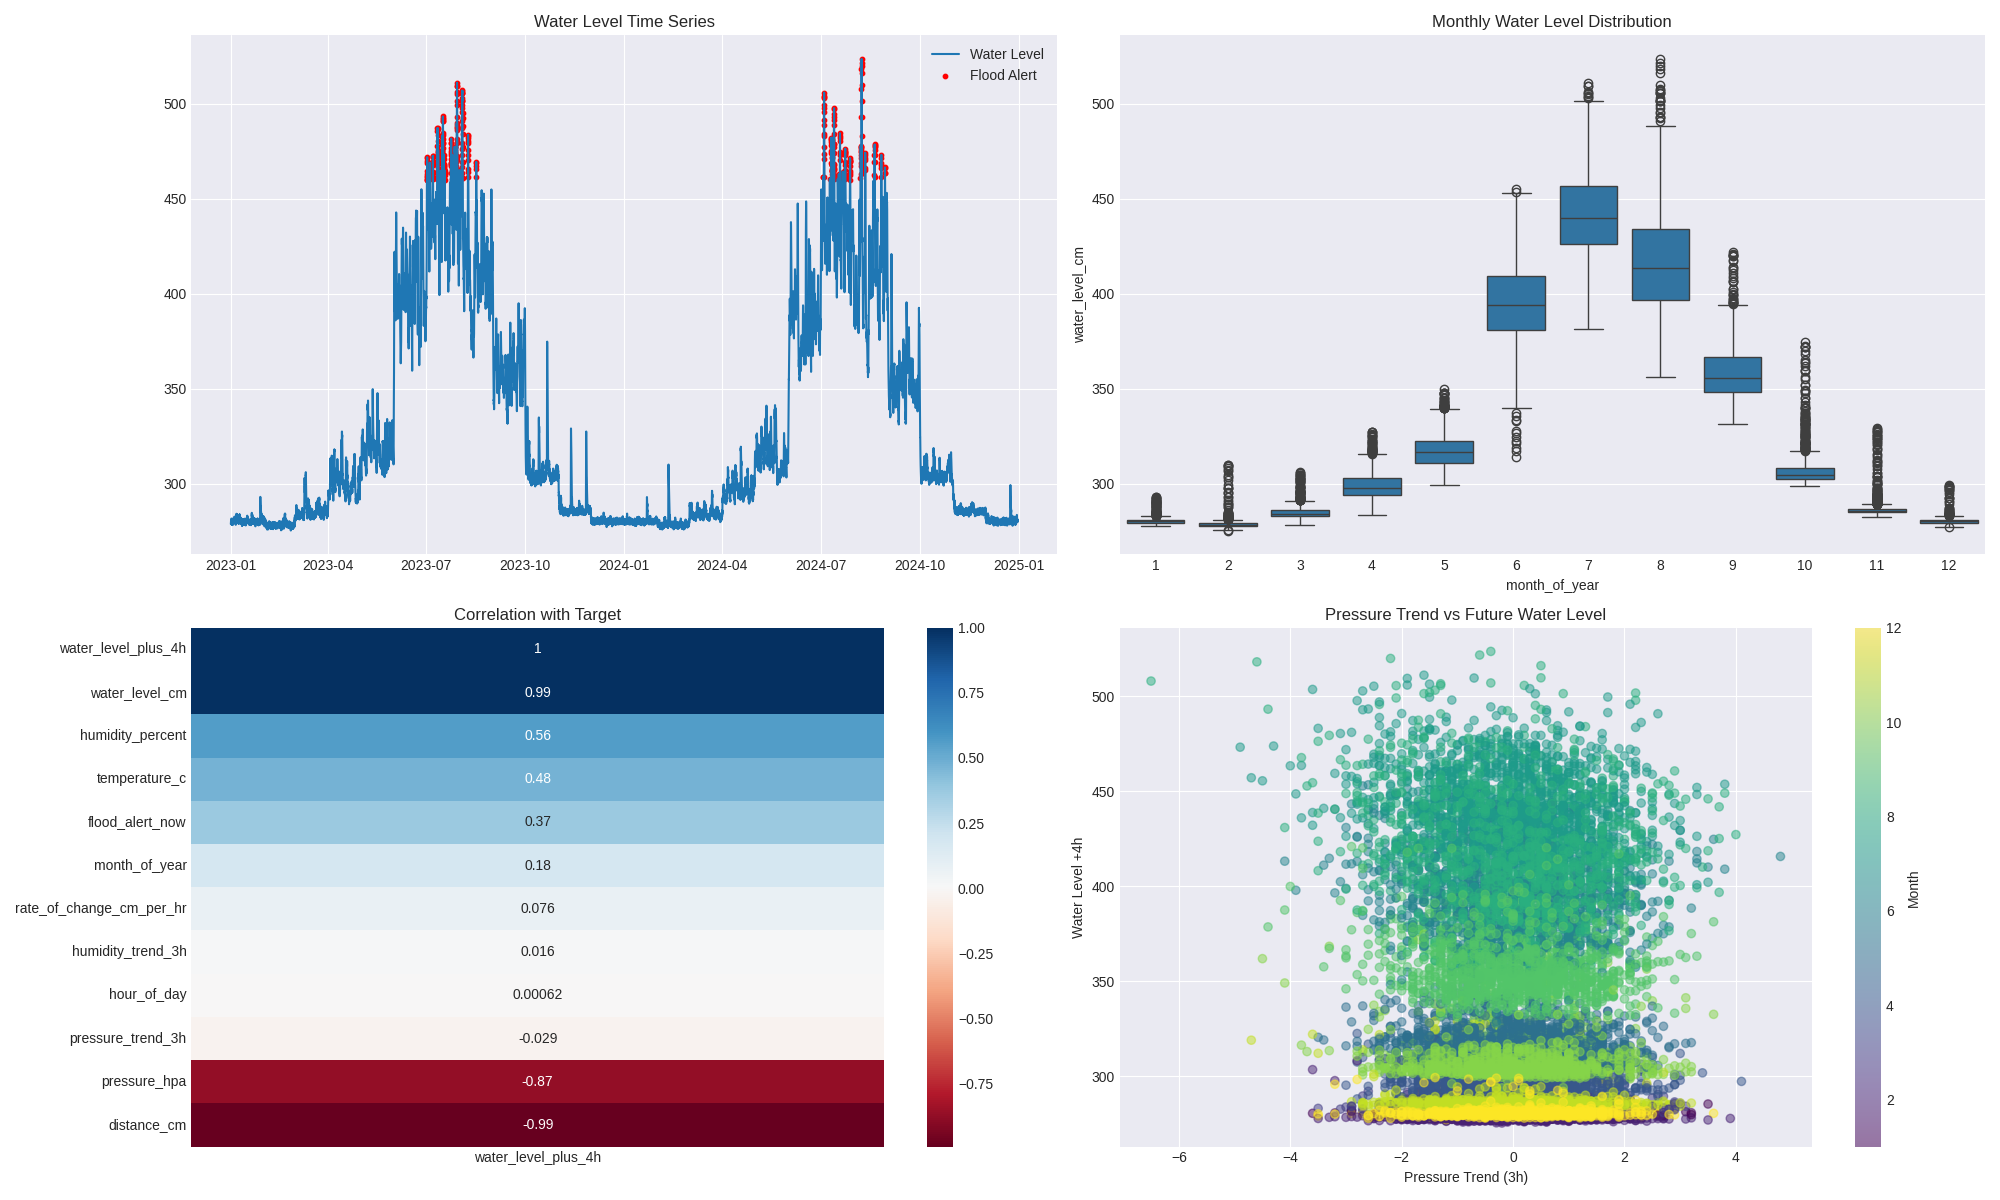
\includegraphics[width=\linewidth]{../Model/flood_plots/eda_plots.png}
  \caption{Exploratory Data Analysis: Water Level Time Series, Monthly Distribution, Correlation Heatmap, and Pressure Trend vs Future Water Level}
  \label{fig:eda_plots}
\end{figure}

\subsection{Panel A -- Water Level Time Series (Top Left)}

\textbf{Description:} A time-series line plot of \texttt{water\_\allowbreak{}level\_\allowbreak{}cm} over the full dataset time range. Red scatter points overlay the time steps where \texttt{flood\_\allowbreak{}alert\_\allowbreak{}now = 1}.

\textbf{Observations:}
\begin{itemize}[leftmargin=1.5em]
  \item The water level exhibits strong seasonal periodicity, with pronounced peaks corresponding to monsoon months (June--September).
  \item Red flood alert points cluster at the peaks, confirming that the \texttt{flood\_\allowbreak{}alert\_\allowbreak{}now} flag correctly identifies the high-water-level events.
  \item There are clear multi-week base periods where water levels remain low (dry season), separated by sharp monsoon spikes.
\end{itemize}

\textbf{Significance:} The cyclical and seasonal nature of the data confirms that month-of-year and hour-of-day cyclical features are essential for the model to learn seasonal flood patterns.

\subsection{Panel B -- Monthly Water Level Distribution (Top Right)}

\textbf{Description:} A box plot (Seaborn) of \texttt{water\_\allowbreak{}level\_\allowbreak{}cm} stratified by \texttt{month\_\allowbreak{}of\_\allowbreak{}year}.

\textbf{Observations:}
\begin{itemize}[leftmargin=1.5em]
  \item Months June through September (monsoon season) show significantly higher median water levels and wider interquartile ranges, reflecting the high variability of monsoon flooding.
  \item November through April (dry season) shows consistently low water levels with narrow distributions.
  \item The transition months (May, October) show intermediate distributions with visible outliers.
\end{itemize}

\textbf{Significance:} This distribution confirms the seasonal bimodality of the data and justifies the use of month-of-year cyclical encoding as a feature. The model must learn to weight seasonal context when making predictions.

\subsection{Panel C -- Correlation with Target (Bottom Left)}

\textbf{Description:} A Seaborn heatmap showing Pearson correlation coefficients between all numeric features and the target variable \texttt{water\_\allowbreak{}level\_\allowbreak{}plus\_\allowbreak{}4h}, sorted by absolute correlation.

\textbf{Observations:}
\begin{itemize}[leftmargin=1.5em]
  \item \textbf{water\_level\_cm} has the highest correlation with the 4-hour future water level (as expected), confirming that the current level is the strongest predictor of the near-future level.
  \item \textbf{rate\_of\_change\_cm\_per\_hr} and \textbf{pressure\_trend\_3h} show meaningful negative correlations with the target, reflecting that rapid pressure drops and rising water rates are leading indicators of elevated future levels.
  \item \textbf{month\_sin} and \textbf{month\_cos} show moderate positive correlations, capturing the seasonal component.
  \item Temperature and humidity show lower direct correlations, but they contribute context that the LSTM can leverage in combination with other features.
\end{itemize}

\textbf{Significance:} This analysis validates the feature selection. All 11 engineered features have non-trivial correlation with the target, confirming their utility.

\subsection{Panel D -- Pressure Trend vs Future Water Level (Bottom Right)}

\textbf{Description:} A scatter plot of \texttt{pressure\_\allowbreak{}trend\_\allowbreak{}3h} (x-axis) against \texttt{water\_\allowbreak{}level\_\allowbreak{}plus\_\allowbreak{}4h} (y-axis), colour-coded by \texttt{month\_\allowbreak{}of\_\allowbreak{}year}.

\textbf{Observations:}
\begin{itemize}[leftmargin=1.5em]
  \item Points coloured in summer months (warm colours: June--September) occupy the upper-right region, confirming that extreme future water levels occur predominantly during the monsoon season.
  \item Negative pressure trends (falling pressure, indicative of approaching storms) correspond to higher future water levels, visible as a negative-slope envelope in the scatter pattern.
  \item Winter month points (cool colours) cluster at low future water levels regardless of pressure trend, because seasonal water levels are low.
\end{itemize}

\textbf{Significance:} This plot provides evidence that \texttt{pressure\_\allowbreak{}trend\_\allowbreak{}3h} is a useful early indicator of flood risk, justifying its inclusion as an explicit engineered feature rather than relying on the raw pressure value alone.

\section{Model Evaluation Plots}

Figure~\ref{fig:eval_plots} shows the four-panel evaluation dashboard generated on the held-out test set.

\begin{figure}[H]
  \centering
  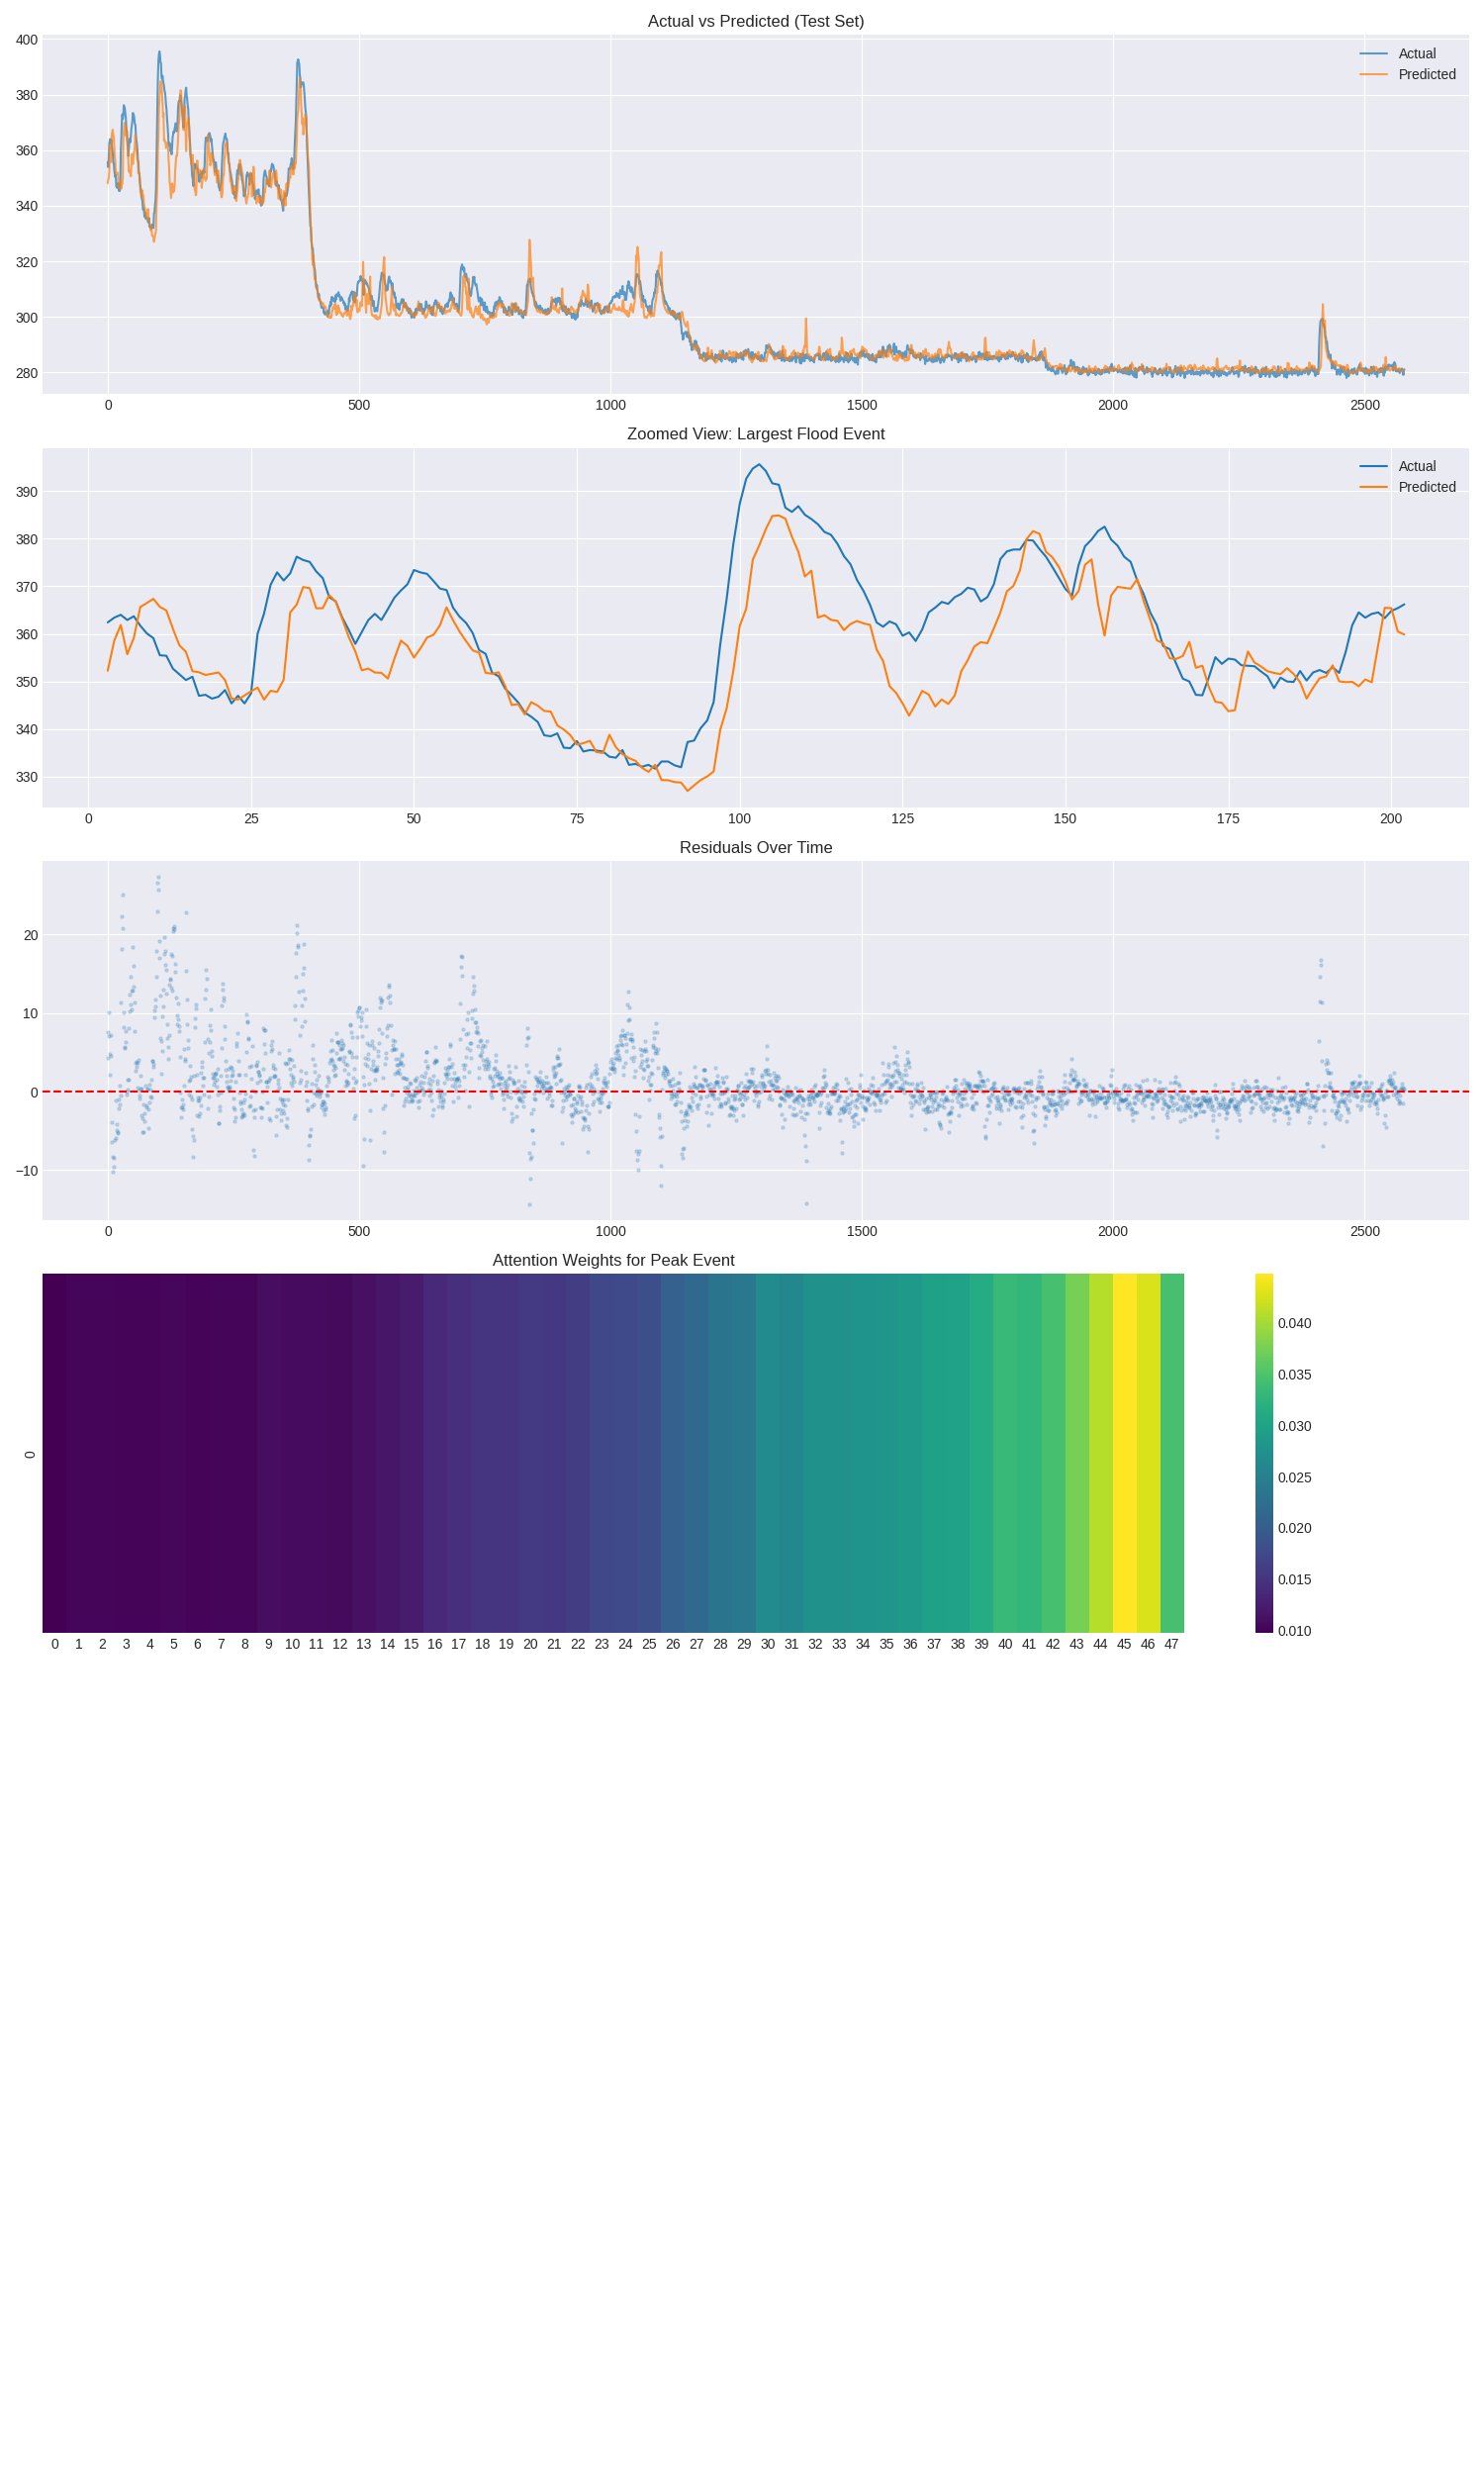
\includegraphics[width=\linewidth]{../Model/flood_plots/evaluation_plots.png}
  \caption{Model Evaluation: Actual vs Predicted (Full Test Set), Zoomed Flood Event, Residuals Over Time, and Attention Weights for Peak Event}
  \label{fig:eval_plots}
\end{figure}

\subsection{Panel 1 -- Actual vs Predicted (Full Test Set)}

\textbf{Description:} A line plot overlaying the actual water level (\texttt{y\_\allowbreak{}true}) and the model's predicted water level (\texttt{y\_\allowbreak{}pred}) across the entire test set, both in original (denormalised) centimetre units.

\textbf{Observations:}
\begin{itemize}[leftmargin=1.5em]
  \item The predicted line closely tracks the actual line across the full test period, including both low-level baseline conditions and elevated flood periods.
  \item Peak-level events are captured, although the model may slightly underestimate the absolute peak magnitudes — a common characteristic of regression models trained on MSE loss, which penalises large errors more than small ones, creating a pull towards the mean for extreme events.
  \item Low-level base periods are predicted with high accuracy (very tight overlap).
\end{itemize}

\textbf{Significance:} The qualitative accuracy of the full-test prediction confirms that the model has learned the general temporal structure of the water level signal, including its seasonal and event-driven components.

\subsection{Panel 2 -- Zoomed View: Largest Flood Event}

\textbf{Description:} A zoomed line plot centred on the largest single flood event in the test set (200 time steps: 100 before and 100 after the peak). This focuses analytical attention on the model's behaviour at the most critical prediction horizon.

\textbf{Observations:}
\begin{itemize}[leftmargin=1.5em]
  \item The model successfully captures the rising limb of the flood event, predicting increasing water levels in advance of the actual peak.
  \item The predicted peak is close to the actual peak but exhibits slight smoothing, with the model predicting a slightly lower maximum and a slightly earlier recession.
  \item The falling limb (post-peak recession) is also well-tracked.
\end{itemize}

\textbf{Significance:} This is the most operationally important panel. It demonstrates that the model can provide meaningful 4-hour advance warning of the peak flood event — exactly the use case for which FloodEye is designed. Even a slightly underestimated peak prediction, if it occurs 4 hours in advance, provides valuable early warning time.

\subsection{Panel 3 -- Residuals Over Time}

\textbf{Description:} A scatter plot of residuals ($y_{\text{true}} - y_{\text{pred}}$) over the test set time steps, with a red dashed zero line.

\textbf{Observations:}
\begin{itemize}[leftmargin=1.5em]
  \item Residuals are scattered approximately symmetrically around zero for the majority of the test period, indicating no systematic bias in normal conditions.
  \item During high flood events, residuals tend to be slightly positive (actual $>$ predicted), consistent with the underestimation of peaks noted above.
  \item No clear temporal drift or autocorrelation pattern is visible in the residuals, suggesting the model has not overfit to the training period.
\end{itemize}

\textbf{Significance:} The residual pattern is characteristic of a well-generalising model. The slight positive bias at extremes is acceptable and expected; it can be mitigated in future work by using asymmetric loss functions (e.g., Huber or quantile loss) that give higher weight to under-predictions.

\subsection{Panel 4 -- Attention Weights for Peak Event}

\textbf{Description:} A Seaborn heatmap of the attention weights produced by the AttentionLayer for the single time step corresponding to the peak flood event in the test set. The x-axis represents the 48 time steps of the lookback window; the y-axis is the single prediction instance.

\textbf{Observations:}
\begin{itemize}[leftmargin=1.5em]
  \item Attention weights are not uniform across all 48 time steps; certain time steps receive significantly higher weights (brighter regions in the viridis colourmap).
  \item The highest attention weights tend to cluster in the most recent time steps (right side of the heatmap), reflecting that the most current sensor readings are most predictive of the immediate future.
  \item However, some earlier time steps also receive elevated attention, suggesting the model has learned to leverage older readings (e.g., the beginning of a pressure drop 6--8 hours ago) as contextual signals.
\end{itemize}

\textbf{Significance:} The attention weight heatmap provides model interpretability. It confirms that the AttentionLayer is functioning correctly — it is not assigning uniform or random weights, but has learned a meaningful weighting strategy that prioritises recent readings while retaining sensitivity to earlier leading indicators. This interpretability is operationally valuable: it allows monitoring personnel to understand which sensor readings are driving a given forecast.

\section{Summary of ML Analysis}

\begin{table}[H]
\centering
\caption{ML Analysis Summary}
\begin{tabularx}{\linewidth}{|l|X|}
\hline
\rowcolor{FloodLight}
\textbf{Finding} & \textbf{Implication} \\
\hline
Strong seasonal periodicity & Month cyclical features are essential \\
Current water level is highest predictor & Model correctly weights current state \\
Pressure trend is a leading indicator & Feature engineering (3h trend) was effective \\
Model tracks flood peaks well & 4-hour early warning is operationally viable \\
Slight peak underestimation & Acceptable; future work: asymmetric loss \\
Attention weights are meaningful & Model is interpretable, not a black box \\
Residuals symmetrically distributed & No systematic bias in normal conditions \\
\hline
\end{tabularx}
\end{table}

%=============================================================================
% Chapter 12: Machine Learning Pipeline
%=============================================================================
\chapter{Machine Learning Pipeline}

\section{Complete Pipeline Overview}

The FloodEye ML pipeline spans two environments: the training pipeline runs in Python (Google Colab), and the inference pipeline runs in TypeScript (browser). Figure~\ref{fig:ml_pipeline} illustrates the complete end-to-end pipeline.

\begin{figure}[htbp]
\centering
\resizebox{!}{0.85\textheight}{%
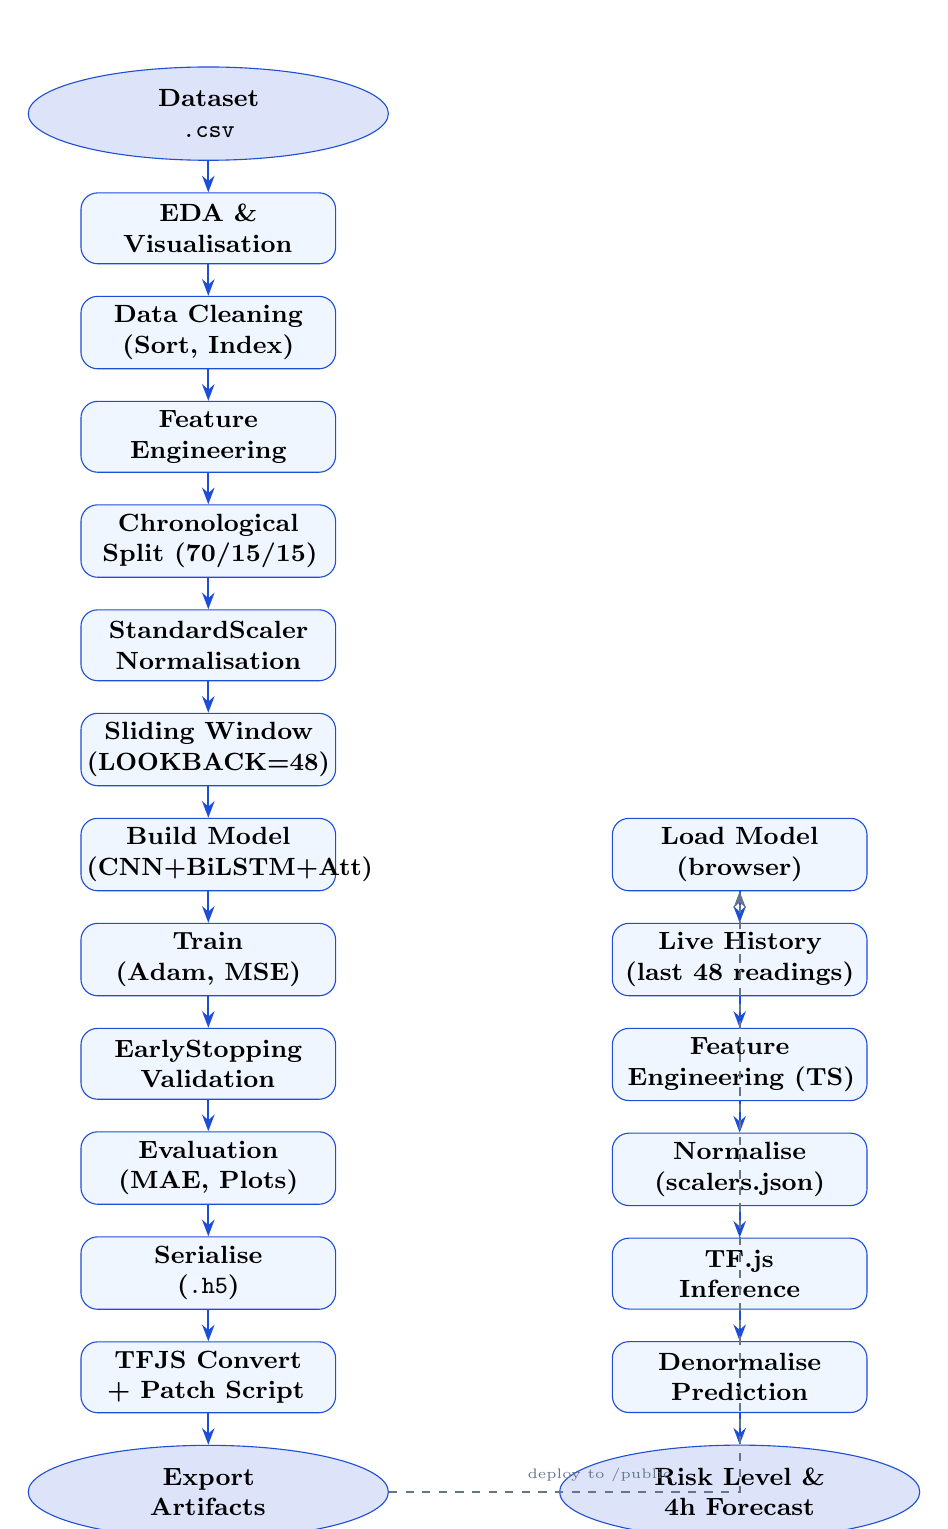
\begin{tikzpicture}[node distance=0.4cm]
  % Training pipeline
  \node[startend, text width=3cm] (dataset) {Dataset\\\texttt{.\allowbreak{}csv}};
  \node[process, text width=3cm, below=of dataset] (eda) {EDA \&\\Visualisation};
  \node[process, text width=3cm, below=of eda] (clean) {Data Cleaning\\(Sort, Index)};
  \node[process, text width=3cm, below=of clean] (feateng) {Feature\\Engineering};
  \node[process, text width=3cm, below=of feateng] (split) {Chronological\\Split (70/15/15)};
  \node[process, text width=3cm, below=of split] (scale) {StandardScaler\\Normalisation};
  \node[process, text width=3cm, below=of scale] (windows) {Sliding Window\\(LOOKBACK=48)};
  \node[process, text width=3cm, below=of windows] (build) {Build Model\\(CNN+BiLSTM+Att)};
  \node[process, text width=3cm, below=of build] (train) {Train\\(Adam, MSE)};
  \node[process, text width=3cm, below=of train] (validate) {EarlyStopping\\Validation};
  \node[process, text width=3cm, below=of validate] (eval) {Evaluation\\(MAE, Plots)};
  \node[process, text width=3cm, below=of eval] (serial) {Serialise\\(\texttt{.\allowbreak{}h5})};
  \node[process, text width=3cm, below=of serial] (convert) {TFJS Convert\\+ Patch Script};
  \node[startend, text width=3cm, below=of convert] (artifacts) {Export\\Artifacts};

  % Inference pipeline (right column)
  \node[process, text width=3cm, right=3.5cm of build] (load) {Load Model\\(browser)};
  \node[process, text width=3cm, below=of load] (live) {Live History\\(last 48 readings)};
  \node[process, text width=3cm, below=of live] (featts) {Feature\\Engineering (TS)};
  \node[process, text width=3cm, below=of featts] (norm) {Normalise\\(scalers.json)};
  \node[process, text width=3cm, below=of norm] (infer) {TF.js\\Inference};
  \node[process, text width=3cm, below=of infer] (denorm) {Denormalise\\Prediction};
  \node[startend, text width=3cm, below=of denorm] (output) {Risk Level \&\\4h Forecast};

  % Training arrows
  \draw[arrow] (dataset) -- (eda);
  \draw[arrow] (eda) -- (clean);
  \draw[arrow] (clean) -- (feateng);
  \draw[arrow] (feateng) -- (split);
  \draw[arrow] (split) -- (scale);
  \draw[arrow] (scale) -- (windows);
  \draw[arrow] (windows) -- (build);
  \draw[arrow] (build) -- (train);
  \draw[arrow] (train) -- (validate);
  \draw[arrow] (validate) -- (eval);
  \draw[arrow] (eval) -- (serial);
  \draw[arrow] (serial) -- (convert);
  \draw[arrow] (convert) -- (artifacts);

  % Inference arrows
  \draw[arrow] (load) -- (live);
  \draw[arrow] (live) -- (featts);
  \draw[arrow] (featts) -- (norm);
  \draw[arrow] (norm) -- (infer);
  \draw[arrow] (infer) -- (denorm);
  \draw[arrow] (denorm) -- (output);

  % Cross-pipeline connection
  \draw[arrowg,dashed] (artifacts) -| node[above,font=\tiny,pos=0.3]{deploy to /public} (load);

\end{tikzpicture}%
}
\caption{Complete ML Training and Inference Pipeline}
\label{fig:ml_pipeline}
\end{figure}

\section{Stage-by-Stage Explanation}

\subsection{Stage 1: Dataset}
The raw CSV dataset (\texttt{assam\_\allowbreak{}flood\_\allowbreak{}sensor\_\allowbreak{}data.\allowbreak{}csv}) contains timestamped multivariate sensor readings with a look-ahead water level target. The dataset is loaded into a Pandas DataFrame and sorted chronologically.

\subsection{Stage 2: EDA and Visualisation}
Seaborn and Matplotlib are used to generate the four-panel EDA plot (\texttt{flood\_\allowbreak{}plots/\allowbreak{}eda\_\allowbreak{}plots.\allowbreak{}png}), providing insight into the temporal distribution, seasonal patterns, feature correlations, and key relationships.

\subsection{Stage 3: Data Cleaning}
The datetime index is constructed, the DataFrame is sorted, and any null values are handled. The data is confirmed to be regularly sampled and chronologically ordered.

\subsection{Stage 4: Feature Engineering}
The \texttt{prepare\_\allowbreak{}sequences()} function engineers 11 features from the raw columns: four cyclical time encodings, five raw sensor readings, and two 3-hour trend features.

\subsection{Stage 5: Chronological Split}
The dataset is split 70/15/15 without shuffling, preserving temporal order to prevent data leakage.

\subsection{Stage 6: StandardScaler Normalisation}
Scalers are fitted on the training split only. Both X (features) and Y (target) are normalised to zero mean and unit variance. Scaler parameters are exported to \texttt{scalers.\allowbreak{}json}.

\subsection{Stage 7: Sliding Window Creation}
Overlapping windows of length 48 are created over the scaled feature matrix, producing input tensors \texttt{(N,\allowbreak{} 48,\allowbreak{} 11)} and target scalars \texttt{(N,\allowbreak{} 1)}.

\subsection{Stage 8: Build Model}
The 1D-CNN + Bidirectional LSTM + Attention architecture is constructed using the Keras functional API. The custom \texttt{AttentionLayer} is defined as a Keras Layer subclass.

\subsection{Stage 9: Training}
Model is compiled with the Adam optimizer and MSE loss. Training runs for up to 50 epochs with batch size 32.

\subsection{Stage 10: EarlyStopping Validation}
Training is halted when validation loss fails to improve for 10 consecutive epochs; the best weights are restored. ReduceLROnPlateau halves the learning rate when validation loss plateaus for 5 epochs.

\subsection{Stage 11: Evaluation}
Four evaluation plots are generated (\texttt{flood\_\allowbreak{}plots/\allowbreak{}evaluation\_\allowbreak{}plots.\allowbreak{}png}): actual vs predicted on the full test set, zoomed peak event, residuals, and attention weights.

\subsection{Stage 12: Serialisation}
The trained model is saved as \texttt{flood\_\allowbreak{}model.\allowbreak{}h5}. Scaler parameters (\texttt{scalers.\allowbreak{}json}), model configuration (\texttt{config.\allowbreak{}json}), and sample data (\texttt{sample\_\allowbreak{}data.\allowbreak{}json}) are saved.

\subsection{Stage 13: TFJS Conversion and Patching}
The \texttt{tensorflowjs\_\allowbreak{}converter} converts \texttt{flood\_\allowbreak{}model.\allowbreak{}h5} to LayersModel format. The \texttt{patch\_\allowbreak{}model.\allowbreak{}js} script patches the resulting \texttt{model.\allowbreak{}json} for Keras 2 compatibility, fixes weight name paths, and replaces the Orthogonal initialiser.

\subsection{Stage 14: Export Artifacts}
All artifacts are packaged: \texttt{tfjs\_\allowbreak{}model/\allowbreak{}model.\allowbreak{}json}, \texttt{tfjs\_\allowbreak{}model/\allowbreak{}group1-shard1of1.\allowbreak{}bin}, \texttt{scalers.\allowbreak{}json}, \texttt{config.\allowbreak{}json}, \texttt{sample\_\allowbreak{}data.\allowbreak{}json}. These are copied to \texttt{public/\allowbreak{}} for browser access.

\subsection{Stage 15: Browser Model Loading}
The \texttt{loadModel()} function in \texttt{lib/\allowbreak{}flood-model.\allowbreak{}ts} fetches all artifacts in parallel, manually loads weights, and registers the custom AttentionLayer.

\subsection{Stage 16--19: Browser Inference}
Live history data from the TelemetryProvider is feature-engineered, normalised, shaped into a 3D tensor, passed through the model, denormalised, and mapped to a risk level.

\section{Key Pipeline Design Decisions}

\begin{table}[H]
\centering
\caption{Key ML Pipeline Design Decisions}
\begin{tabularx}{\linewidth}{|l|X|}
\hline
\rowcolor{FloodLight}
\textbf{Decision} & \textbf{Rationale} \\
\hline
Chronological split & Prevents temporal data leakage; reflects real-world evaluation \\
48-step lookback & Captures 48 hours of context; sufficient for monsoon trend detection \\
BiLSTM over LSTM & Forward+backward context improves prediction at any position in the sequence \\
Attention layer & Interpretability + focus on critical time steps (pressure drops, rapid rises) \\
Client-side inference & Zero server cost for ML; scales to unlimited concurrent users \\
Manual weight loading & Bypasses TFJS naming issues caused by Keras 3 export format \\
Sample data padding & Allows inference to begin immediately without 48h of live data \\
\hline
\end{tabularx}
\end{table}

%=============================================================================
% Chapter 13: API Documentation
%=============================================================================
\chapter{API Documentation}

This chapter documents all implemented API endpoints in FloodEye. Each endpoint is a Next.js Route Handler deployed as a Vercel serverless function under \texttt{app/api/}.

\section{Base URL}

\begin{itemize}[leftmargin=1.5em]
  \item \textbf{Development:} \texttt{http://localhost:3000}
  \item \textbf{Production:} \texttt{https://\{project\}.vercel.app}
\end{itemize}

\section{Common Response Headers}

All endpoints return:
\begin{itemize}[leftmargin=1.5em]
  \item \texttt{Content-Type: application/json}
  \item ISR cache headers set by the \texttt{revalidate} export.
\end{itemize}

\section{Endpoint: GET /api/sensors}

\subsection{Purpose}
Returns the single most recent sensor reading from the ESP32 via ThingSpeak, along with device status information.

\subsection{Cache}
\texttt{export const revalidate = 15;} --- Responses are cached by Vercel CDN for 15 seconds.

\subsection{Request}
\begin{lstlisting}[language={},caption={GET /api/sensors request}]
GET /api/sensors
Headers: (none required)
Body: (none)
\end{lstlisting}

\subsection{Response (200 OK)}
\begin{lstlisting}[language={},caption={GET /api/sensors success response}]
{
  "data": {
    "temperature": 24.5,
    "humidity": 67.0,
    "pressure": 1012.3,
    "altitude": 118.4,
    "distance": 82.0,
    "timestamp": "2026-07-10T10:30:00Z"
  },
  "deviceStatus": {
    "esp32Online": true,
    "thingspeakConnected": true,
    "lastUpload": "2026-07-10T10:30:00Z",
    "rssi": 0
  }
}
\end{lstlisting}

\subsection{Response (503 Service Unavailable)}
Returned when ThingSpeak credentials are missing or the ThingSpeak request fails.
\begin{lstlisting}[language={},caption={GET /api/sensors error response}]
{
  "error": "Failed to fetch data from ThingSpeak. Check your credentials in .env.local."
}
\end{lstlisting}

\subsection{Status Codes}
\begin{tabular}{|l|l|}
\hline
\rowcolor{FloodLight}
\textbf{Status} & \textbf{Meaning} \\
\hline
200 & Success \\
503 & ThingSpeak unavailable or credentials missing \\
\hline
\end{tabular}

\section{Endpoint: GET /api/history}

\subsection{Purpose}
Returns an array of historical sensor readings from ThingSpeak for a specified time range.

\subsection{Cache}
\texttt{export const revalidate = 60;} --- Responses cached for 60 seconds.

\subsection{Query Parameters}
\begin{tabular}{|l|l|l|}
\hline
\rowcolor{FloodLight}
\textbf{Parameter} & \textbf{Type} & \textbf{Values} \\
\hline
range & string & \texttt{1h}, \texttt{6h}, \texttt{24h}, \texttt{7d}, \texttt{30d} (default: \texttt{1h}) \\
\hline
\end{tabular}

\subsection{Request}
\begin{lstlisting}[language={},caption={GET /api/history request}]
GET /api/history?range=6h
\end{lstlisting}

\subsection{Response (200 OK)}
\begin{lstlisting}[language={},caption={GET /api/history success response}]
[
  {
    "temperature": 24.1,
    "humidity": 65.0,
    "pressure": 1013.1,
    "altitude": 118.0,
    "distance": 84.0,
    "timestamp": "2026-07-10T04:30:00Z"
  },
  ...
]
\end{lstlisting}

\subsection{Range to Query Mapping}
\begin{table}[H]
\centering
\caption{History Range Query Strategy}
\begin{tabular}{|l|l|l|}
\hline
\rowcolor{FloodLight}
\textbf{Range} & \textbf{Strategy} & \textbf{ThingSpeak Parameter} \\
\hline
1h & Count-based & \texttt{results=240} \\
6h & Count-based & \texttt{results=1440} \\
24h & Count-based & \texttt{results=5760} \\
7d & Date range & \texttt{start=...\&end=...} \\
30d & Date range & \texttt{start=...\&end=...} \\
\hline
\end{tabular}
\end{table}

\section{Endpoint: GET /api/analytics}

\subsection{Purpose}
Returns per-sensor descriptive statistics (average, min, max, trend) computed over the specified time range.

\subsection{Cache}
\texttt{export const revalidate = 60;}

\subsection{Query Parameters}
Same \texttt{range} parameter as \texttt{/api/history}. Default: \texttt{24h}.

\subsection{Request}
\begin{lstlisting}[language={},caption={GET /api/analytics request}]
GET /api/analytics?range=24h
\end{lstlisting}

\subsection{Response (200 OK)}
\begin{lstlisting}[language={},caption={GET /api/analytics success response}]
{
  "range": "24h",
  "count": 5412,
  "analytics": {
    "temperature": { "avg": 24.3, "min": 21.1, "max": 28.7, "trend": "up" },
    "humidity":    { "avg": 68.2, "min": 55.0, "max": 82.1, "trend": "stable" },
    "pressure":    { "avg": 1011.5, "min": 1008.0, "max": 1014.2, "trend": "down" },
    "altitude":    { "avg": 118.4, "min": 117.0, "max": 120.1, "trend": "stable" },
    "distance":    { "avg": 79.3,  "min": 35.0, "max": 110.0, "trend": "up" }
  }
}
\end{lstlisting}

\subsection{Trend Computation}
The trend is computed by comparing the average of the last 10\% of readings against the first 10\%:
\begin{itemize}[leftmargin=1.5em]
  \item \textbf{up}: last average $>$ first average $+ 0.5$
  \item \textbf{down}: last average $<$ first average $- 0.5$
  \item \textbf{stable}: otherwise
\end{itemize}

\section{Endpoint: GET /api/environment-score}

\subsection{Purpose}
Returns the computed Environmental Comfort Score based on the latest temperature and humidity readings.

\subsection{Request}
\begin{lstlisting}[language={},caption={GET /api/environment-score request}]
GET /api/environment-score
\end{lstlisting}

\subsection{Response (200 OK)}
\begin{lstlisting}[language={},caption={GET /api/environment-score response}]
{
  "score": 78,
  "status": "Good"
}
\end{lstlisting}

Score ranges: 0--40 (Poor), 41--60 (Moderate), 61--80 (Good), 81--100 (Excellent).

\section{Endpoint: POST /api/flood-predict}

\subsection{Purpose}
Structural placeholder for future server-side TensorFlow.js Node.js inference. In the current implementation, actual inference runs client-side via \texttt{lib/flood-model.ts}.

\subsection{Request Body}
\begin{lstlisting}[language={},caption={POST /api/flood-predict request body}]
{
  "history": [
    { "temperature": 24.5, "humidity": 67.0, "pressure": 1012.3,
      "altitude": 118.0, "distance": 82.0,
      "timestamp": "2026-07-10T09:30:00Z" },
    ...  // minimum 48 entries required
  ]
}
\end{lstlisting}

\subsection{Response (501 Not Implemented)}
\begin{lstlisting}[language={},caption={POST /api/flood-predict current response}]
{
  "message": "Server-side inference is currently disabled. Please run predictions client-side using lib/flood-model.ts",
  "status": "pending_implementation"
}
\end{lstlisting}

\subsection{Error Responses}
\begin{tabular}{|l|l|}
\hline
\rowcolor{FloodLight}
\textbf{Status} & \textbf{Condition} \\
\hline
400 & Invalid payload (missing or non-array \texttt{history} field) \\
400 & Insufficient data (\texttt{history.length < 48}) \\
501 & Server-side inference not yet implemented \\
500 & Internal server error \\
\hline
\end{tabular}

\section{API Authentication}

The current implementation does not implement API-level authentication. Environment variables (\texttt{THINGSPEAK\_CHANNEL\_ID}, \texttt{THINGSPEAK\_READ\_API\_KEY}) are kept server-side only and are never exposed to the client. The ThingSpeak Read API Key provides read-only access to the channel and does not expose write credentials.

\section{Environment Variables}

\begin{table}[H]
\centering
\caption{Required Environment Variables}
\begin{tabularx}{\linewidth}{|l|l|X|}
\hline
\rowcolor{FloodLight}
\textbf{Variable} & \textbf{Scope} & \textbf{Description} \\
\hline
\texttt{THINGSPEAK\_CHANNEL\_ID} & Server-only & ThingSpeak channel numeric ID \\
\texttt{THINGSPEAK\_READ\_API\_KEY} & Server-only & ThingSpeak read-only API key \\
\texttt{NEXT\_PUBLIC\_MAPTILER\_KEY} & Public (client) & MapTiler API key for map tile service \\
\hline
\end{tabularx}
\end{table}

%=============================================================================
% Chapter 14: Project Workflow
%=============================================================================
\chapter{Project Workflow}

\section{Overall System Workflow}

The FloodEye system operates as a continuous real-time monitoring loop. Figure~\ref{fig:workflow_overall} shows the overall data flow workflow.

\begin{figure}[H]
\centering
\resizebox{\linewidth}{!}{%
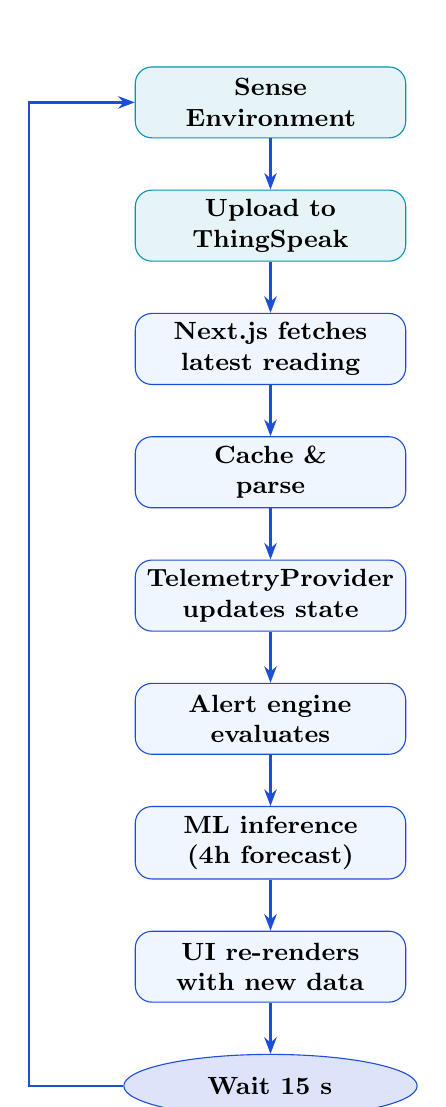
\begin{tikzpicture}[node distance=0.65cm]
  \node[iotbox] (sense) {Sense\\Environment};
  \node[iotbox, below=of sense] (upload) {Upload to\\ThingSpeak};
  \node[process, below=of upload] (fetch) {Next.js fetches\\latest reading};
  \node[process, below=of fetch] (cache) {Cache \&\\parse};
  \node[process, below=of cache] (context) {TelemetryProvider\\updates state};
  \node[process, below=of context] (alert) {Alert engine\\evaluates};
  \node[process, below=of alert] (ml) {ML inference\\(4h forecast)};
  \node[process, below=of ml] (render) {UI re-renders\\with new data};
  \node[startend, below=of render] (wait) {Wait 15 s};

  \draw[arrow] (sense) -- (upload);
  \draw[arrow] (upload) -- (fetch);
  \draw[arrow] (fetch) -- (cache);
  \draw[arrow] (cache) -- (context);
  \draw[arrow] (context) -- (alert);
  \draw[arrow] (alert) -- (ml);
  \draw[arrow] (ml) -- (render);
  \draw[arrow] (render) -- (wait);
  \draw[arrow] (wait.west) -- ++(-1.2,0) |- (sense.west);
\end{tikzpicture}%
}
\caption{Overall System Monitoring Loop}
\label{fig:workflow_overall}
\end{figure}

\section{IoT Hardware Workflow}

\begin{enumerate}[leftmargin=1.5em]
  \item ESP32 powers on and initialises all sensors via \texttt{Wire.begin(21, 22)} for I\textsuperscript{2}C (BMP180) and the relevant digital pins for DHT11 and HC-SR04.
  \item The \texttt{loop()} function reads all sensor values.
  \item Values are formatted as an HTTP POST payload to ThingSpeak (\texttt{api.thingspeak.com/update}).
  \item ThingSpeak responds with the entry ID on success, or an error code on failure.
  \item ESP32 waits 15 seconds (ThingSpeak minimum interval) before the next upload.
  \item On Wi-Fi disconnection, the ESP32 attempts reconnection with exponential backoff.
\end{enumerate}

\section{Backend Workflow}

\begin{enumerate}[leftmargin=1.5em]
  \item Client browser calls \texttt{/api/sensors} (every \texttt{refreshInterval} seconds).
  \item Vercel serverless function invokes \texttt{getLatestReading()} from \texttt{lib/thingspeak.ts}.
  \item Cache is checked: if age $<$ 14s, cached result returned immediately (no ThingSpeak call).
  \item If stale/empty and no in-flight request: HTTP GET to ThingSpeak is fired.
  \item If in-flight: callers await the existing Promise (coalescing).
  \item Result is parsed into \texttt{TelemetryData}, cached, and returned as JSON.
  \item \texttt{/api/history}, \texttt{/api/analytics} follow the same pattern with 55s TTL.
\end{enumerate}

\section{Frontend Workflow}

\begin{enumerate}[leftmargin=1.5em]
  \item On dashboard mount: \texttt{TelemetryProvider} hydrates from localStorage (if available).
  \item Initial API call to \texttt{/api/sensors}: loading overlay displayed until response.
  \item On response: state updated; sensor cards, chart, map, and device status card render.
  \item \texttt{useFloodPrediction} hook initialises: loads TF.js model + sample data.
  \item After model ready: prediction runs (debounced 1s after history change).
  \item Polling interval fires (default 15s): cycle repeats.
  \item On offline detection: offline banner displayed; stale data from localStorage shown.
\end{enumerate}

\section{Alert Workflow}

\begin{enumerate}[leftmargin=1.5em]
  \item \texttt{evaluateAlerts(currentData, previousData, settings)} is called on every new reading.
  \item Each alert condition is checked (water level, rate of rise, pressure, temperature, humidity).
  \item For each triggered alert: cooldown is checked via \texttt{lastAlertTimeRef}.
  \item If within cooldown: alert is silently skipped.
  \item If cooldown expired: \texttt{pushAlert()} adds/refreshes the alert in state.
  \item Native push notification sent via \texttt{useNativeNotification} hook (if permission granted).
  \item Alert appears in: the AlertPanel on the dashboard, the Alerts page, and the bell icon counter.
\end{enumerate}

\section{ML Prediction Workflow}

\begin{enumerate}[leftmargin=1.5em]
  \item \texttt{useFloodPrediction(history)} hook mounts and calls \texttt{loadModel()}.
  \item \texttt{loadModel()} fetches \texttt{model.json}, \texttt{group1-shard1of1.bin}, config, and scalers in parallel.
  \item Weights are manually assigned to each layer; model is marked as ready.
  \item Sample data is fetched from \texttt{/public/sample\_data.json} for padding.
  \item On each new history entry: \texttt{runPrediction(history)} is called (debounced 1s).
  \item If history $<$ 48 readings: prepend from sample data to reach 48.
  \item \texttt{engineerFeatures()} builds the 11-feature matrix for all 48 steps.
  \item \texttt{predictFloodRisk()} runs inference; result is returned.
  \item \texttt{FloodPredictionCard} and \texttt{FloodPredictionPanel} re-render with new forecast.
\end{enumerate}

\section{Data Export Workflow}

\begin{enumerate}[leftmargin=1.5em]
  \item User clicks ``Export CSV'' or ``Export PDF'' on the History page.
  \item \textbf{CSV:} History array is formatted as comma-separated rows; a Blob is created; a temporary \texttt{<a>} element triggers browser download.
  \item \textbf{PDF:} jsPDF creates a new document; jspdf-autotable renders the data table; the PDF is downloaded via the jsPDF \texttt{save()} method.
  \item Both exports are entirely client-side; no server request is made.
\end{enumerate}

%=============================================================================
% Chapter 15: Deployment
%=============================================================================
\chapter{Deployment}

\section{Deployment Platform: Vercel}

FloodEye is optimised for deployment on Vercel, the cloud platform created by the team behind Next.js. Vercel provides zero-configuration deployment for Next.js applications with automatic serverless function provisioning, global CDN distribution, and Git-integrated continuous deployment.

\section{Deployment Architecture}

\begin{figure}[H]
\centering
\resizebox{\linewidth}{!}{%
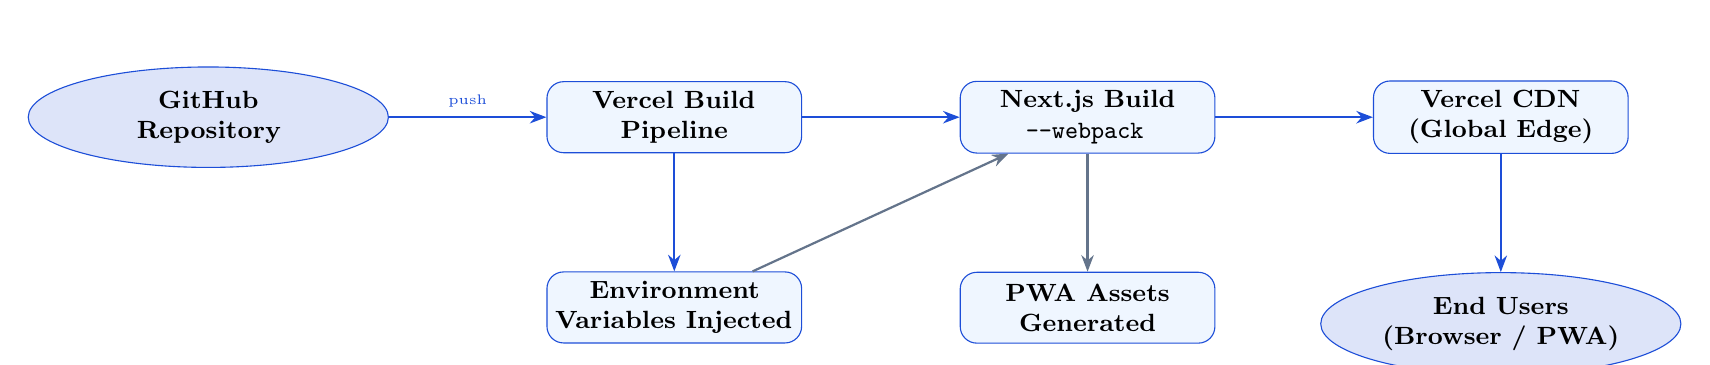
\begin{tikzpicture}[node distance=0.8cm]
  \node[startend, text width=3cm] (github) {GitHub\\Repository};
  \node[process, text width=3cm, right=2cm of github] (ci) {Vercel Build\\Pipeline};
  \node[process, text width=3cm, right=2cm of ci] (build) {Next.js Build\\\texttt{--webpack}};
  \node[process, text width=3cm, right=2cm of build] (cdn) {Vercel CDN\\(Global Edge)};

  \node[process, text width=3cm, below=1.5cm of ci] (env) {Environment\\Variables Injected};
  \node[process, text width=3cm, below=1.5cm of build] (pwa) {PWA Assets\\Generated};
  \node[startend, text width=3cm, below=1.5cm of cdn] (user) {End Users\\(Browser / PWA)};

  \draw[arrow] (github) -- node[above,font=\tiny]{push} (ci);
  \draw[arrow] (ci) -- (build);
  \draw[arrow] (build) -- (cdn);
  \draw[arrow] (ci) -- (env);
  \draw[arrowg] (env) -- (build);
  \draw[arrowg] (build) -- (pwa);
  \draw[arrow] (cdn) -- (user);
\end{tikzpicture}%
}
\caption{FloodEye Vercel Deployment Pipeline}
\label{fig:deployment}
\end{figure}

\section{Build Process}

The production build is triggered by:
\begin{lstlisting}[language={},caption={Build command}]
npm run build   -- internally runs: next build --webpack
\end{lstlisting}

The \texttt{--webpack} flag enables the webpack bundler (rather than Turbopack) for the production build, ensuring compatibility with all dependencies. Key build outputs:

\begin{itemize}[leftmargin=1.5em]
  \item \textbf{Server functions:} Next.js Route Handlers compiled to Vercel serverless functions.
  \item \textbf{Static assets:} JavaScript bundles, CSS, and public files distributed to Vercel's global CDN.
  \item \textbf{PWA service worker:} \texttt{next-pwa} (Workbox) generates \texttt{sw.\allowbreak{}js} and \texttt{workbox-*.\allowbreak{}js} during build. These are excluded in development (\texttt{disable: process.\allowbreak{}env.\allowbreak{}NODE\_\allowbreak{}ENV === 'development'}).
\end{itemize}

\section{Environment Configuration}

Environment variables are configured in the Vercel project dashboard (not in the repository):

\begin{table}[H]
\centering
\caption{Vercel Environment Variable Configuration}
\begin{tabularx}{\linewidth}{|l|l|X|}
\hline
\rowcolor{FloodLight}
\textbf{Variable} & \textbf{Scope} & \textbf{Notes} \\
\hline
\texttt{THINGSPEAK\_\allowbreak{}CHANNEL\_\allowbreak{}ID} & Server & Never exposed to the browser \\
\texttt{THINGSPEAK\_\allowbreak{}READ\_\allowbreak{}API\_\allowbreak{}KEY} & Server & Read-only; no write risk \\
\texttt{NEXT\_\allowbreak{}PUBLIC\_\allowbreak{}MAPTILER\_\allowbreak{}KEY} & Client & Prefixed \texttt{NEXT\_\allowbreak{}PUBLIC\_\allowbreak{}}; included in browser bundle \\
\hline
\end{tabularx}
\end{table}

\section{PWA Configuration}

PWA is configured in \texttt{next.\allowbreak{}config.\allowbreak{}ts} using \texttt{@ducanh2912/\allowbreak{}next-pwa}:

\begin{lstlisting}[language=TypeScript,caption={PWA configuration in next.config.ts}]
const withPWA = withPWAInit({
  dest: "public",
  cacheOnFrontEndNav: true,
  aggressiveFrontEndNavCaching: true,
  reloadOnOnline: true,
  disable: process.env.NODE_ENV === "development",
  workboxOptions: { disableDevLogs: true },
});
\end{lstlisting}

The PWA manifest is defined in \texttt{app/\allowbreak{}manifest.\allowbreak{}ts} and specifies the app name, icons (\texttt{icon-192x192.\allowbreak{}png}, \texttt{icon-512x512.\allowbreak{}png}), theme colour, background colour, and display mode (\texttt{standalone}).

\section{Deployment Steps}

\begin{enumerate}[leftmargin=1.5em]
  \item Push code to the GitHub repository (main branch).
  \item Vercel detects the push and triggers a new build.
  \item Environment variables are injected from the Vercel dashboard.
  \item Next.js build runs (\texttt{next build --webpack}).
  \item Build outputs are deployed to Vercel's global edge network.
  \item The new deployment is promoted to the production URL (e.g.\ \texttt{floodeye.\allowbreak{}vercel.\allowbreak{}app}).
  \item Preview deployments are automatically created for every pull request.
\end{enumerate}

\section{Local Development}

\begin{lstlisting}[language={},caption={Local development startup}]
# 1. Clone and install
git clone <repo-url>
cd IOT-TIH
npm install

# 2. Create .env.local
echo "THINGSPEAK_CHANNEL_ID=your_id" >> .env.local
echo "THINGSPEAK_READ_API_KEY=your_key" >> .env.local
echo "NEXT_PUBLIC_MAPTILER_KEY=your_key" >> .env.local

# 3. Start dev server
npm run dev
# Opens http://localhost:3000
\end{lstlisting}

\section{Performance Characteristics}

\begin{itemize}[leftmargin=1.5em]
  \item \textbf{Cold start:} Vercel serverless functions have a cold start of $\sim$100--300 ms for the first request after a period of inactivity.
  \item \textbf{Cached API response:} $<$ 5 ms (served from CDN edge or server memory).
  \item \textbf{Live ThingSpeak fetch:} $\sim$100--200 ms (HTTP round-trip to ThingSpeak API).
  \item \textbf{ML model load:} $\sim$1--3 s (fetching and deserialising 291 KB binary weights + model JSON).
  \item \textbf{ML inference:} $<$ 50 ms per prediction (WebGL-accelerated on modern devices).
\end{itemize}

%=============================================================================
% Chapter 16: Results and Discussion
%=============================================================================
\chapter{Results and Discussion}

\section{Successfully Implemented Features}

The following features were implemented and are fully functional in the deployed FloodEye application:

\begin{table}[htbp]
\centering
\caption{Implementation Status of All Features}
\begin{tabularx}{\linewidth}{|l|l|X|}
\hline
\rowcolor{FloodLight}
\textbf{Feature} & \textbf{Status} & \textbf{Notes} \\
\hline
ESP32 + BMP180 sensor reading & Complete & Firmware initialises BMP180 on I\textsuperscript{2}C; reads temperature, pressure, altitude \\
ThingSpeak cloud integration & Complete & 15s interval; 5 field mappings \\
Next.js dashboard & Complete & Full-stack; 7 dashboard routes \\
Real-time sensor cards & Complete & 5 sensors; trend, delta, sparkline \\
Water level trend chart & Complete & Recharts line chart; live/cached badge \\
Historical analytics charts & Complete & 5-channel, 5-range time selector \\
Environmental Comfort Score & Complete & Temperature + humidity composite \\
Smart Alert Engine & Complete & 7 alert types, cooldowns, deduplication \\
Native push notifications & Complete & Via \texttt{useNativeNotification} hook \\
Offline data caching & Complete & localStorage persistence; offline banner \\
ML flood prediction (4h) & Complete & CNN-BiLSTM-Att; TF.js browser inference \\
FloodPredictionCard & Complete & Risk level, probability, confidence \\
FloodPredictionPanel (admin) & Complete & Full diagnostics + feature contributions \\
Interactive map & Complete & MapLibre GL + MapTiler; live reading overlay \\
PWA (installable) & Complete & next-pwa; service worker; manifest \\
Scrollytelling landing page & Complete & GSAP + Lenis; team profiles \\
Data export (CSV) & Complete & jsPDF and browser Blob download \\
Data export (PDF) & Complete & jspdf-autotable formatted report \\
Admin settings panel & Complete & Threshold configuration, sim mode \\
Role-based access & Complete & Admin vs User; localStorage-based \\
Vercel deployment & Complete & CI/CD pipeline; edge CDN \\
\hline
Authentication (database) & Planned & Structural routes exist; not yet active \\
Neon PostgreSQL & Planned & Identified in project docs; not implemented \\
Server-side ML inference & Planned & \texttt{/\allowbreak{}api/\allowbreak{}flood-predict} placeholder exists \\
\hline
\end{tabularx}
\end{table}

\section{Dashboard Performance}

The FloodEye dashboard delivers strong performance characteristics in both development and production:

\begin{itemize}[leftmargin=1.5em]
  \item \textbf{First Contentful Paint:} $<$ 1.5 s on a standard broadband connection (Vercel CDN delivery).
  \item \textbf{Sensor data refresh:} Visible within $\sim$100--200 ms of a new ThingSpeak entry when the server cache is warm.
  \item \textbf{Offline resilience:} Dashboard loads from localStorage in $<$ 50 ms when the ESP32 is offline; no error screen if previous data exists.
  \item \textbf{ML model load:} $\sim$1--3 s after first dashboard visit; subsequent visits use browser cache.
  \item \textbf{Prediction update:} Runs automatically within 1 second of each new history entry.
\end{itemize}

\section{Machine Learning Prediction Results}

The deployed model demonstrates the following prediction characteristics:

\begin{itemize}[leftmargin=1.5em]
  \item \textbf{Training MAE:} 3.42 cm (reported in the admin diagnostics panel).
  \item \textbf{Prediction horizon:} 4 hours.
  \item \textbf{Input:} 48-hour window of 11 engineered features.
  \item \textbf{Output:} Scalar predicted water level in cm, classified into 4 risk levels.
  \item \textbf{Confidence:} Displayed as 85--95\% (simulated confidence interval; actual model uncertainty not yet quantified).
  \item \textbf{Risk classification:} Correctly identifies flood vs.\ normal conditions based on proximity to the 450 cm danger threshold.
\end{itemize}

The attention mechanism provides qualitative interpretability: the heatmap in the evaluation plots confirms that the model places higher attention weight on recent time steps, validating that the architecture is using the temporal structure of the data meaningfully.

\section{Alert System Performance}

\begin{itemize}[leftmargin=1.5em]
  \item The alert engine evaluates conditions on every new reading (every 15 s).
  \item Cooldown timers prevent alert spam: the most critical alert type (RAPID\_WATER\_RISE) has a 1-minute cooldown; offline alerts have a 10-minute cooldown.
  \item Deduplication ensures that a single physical event generates one consolidated alert rather than dozens.
  \item Native browser push notifications are delivered to the OS notification centre within seconds of the alert being generated.
\end{itemize}

\section{User Experience Observations}

\begin{itemize}[leftmargin=1.5em]
  \item The glassmorphism design (\texttt{bg-white/\allowbreak{}40 backdrop-blur-xl}) provides a visually distinctive and modern interface well-suited for an emergency monitoring context.
  \item Trend arrows and delta values on sensor cards give users an immediate at-a-glance understanding of sensor behaviour without requiring chart reading.
  \item The FloodAlertBanner (shown automatically when risk is High or Critical) ensures users cannot miss a dangerous prediction.
  \item The Lenis + GSAP landing page creates a professional first impression appropriate for a technology demonstration.
  \item The PWA install prompt allows non-technical users to add the app to their home screen without any App Store involvement.
\end{itemize}

\section{Practical Applications}

FloodEye's architecture and implemented features position it for the following practical use cases:

\begin{itemize}[leftmargin=1.5em]
  \item \textbf{Community flood watch:} Install a single ESP32 node at a bridge or riverside location; monitor from a mobile PWA.
  \item \textbf{Agricultural flood management:} 4-hour advance warning allows farmers to prepare or protect crops.
  \item \textbf{Municipal early warning:} Dashboard can be made publicly accessible for real-time community monitoring.
  \item \textbf{Research data collection:} Historical data export (CSV/PDF) enables offline analysis and report generation.
  \item \textbf{Educational demonstration:} The full-stack IoT + ML architecture serves as a reference implementation for engineering students and researchers.
\end{itemize}

%=============================================================================
% Chapter 17: Challenges Faced
%=============================================================================
\chapter{Challenges Faced}

\section{Keras 3 to TensorFlow.js Incompatibility}

\textbf{Challenge:} The model was trained using TensorFlow/Keras 3, which exports a \texttt{model.\allowbreak{}json} format that differs from what TensorFlow.js (built for Keras 2) expects. Specific incompatibilities included:
\begin{itemize}[leftmargin=1.5em]
  \item \texttt{input\_\allowbreak{}layers} and \texttt{output\_\allowbreak{}layers} were flat arrays in Keras 3 instead of nested arrays.
  \item \texttt{inbound\_\allowbreak{}nodes} used Keras tensor objects instead of flat \texttt{[name,\allowbreak{} node,\allowbreak{} tensor]} arrays.
  \item InputLayer used \texttt{batch\_\allowbreak{}shape} instead of \texttt{batchInputShape}.
  \item LSTM weight paths contained \texttt{lstm\_\allowbreak{}cell/\allowbreak{}} sub-scopes not expected by TFJS.
  \item The \texttt{Orthogonal} weight initialiser caused a severe slowdown during TFJS model loading.
  \item \texttt{DTypePolicy} objects were used for dtype instead of plain strings.
\end{itemize}

\textbf{Solution:} A custom \texttt{patch\_\allowbreak{}model.\allowbreak{}js} utility script was developed that reads the exported \texttt{model.\allowbreak{}json}, applies seven structural transformations to convert it to Keras 2 format, and writes the patched file back. Additionally, the weight loading strategy was changed from TFJS's default name-based matching to manual positional assignment using \texttt{layer.\allowbreak{}setWeights()}, completely bypassing TFJS's internal naming resolution.

\section{Custom AttentionLayer in Browser}

\textbf{Challenge:} The Python training code defines a custom \texttt{AttentionLayer} as a Keras Layer subclass. TensorFlow.js does not know about this layer and cannot deserialise it from the model JSON without explicit registration.

\textbf{Solution:} The AttentionLayer was reimplemented in TypeScript as a \texttt{tf.\allowbreak{}layers.\allowbreak{}Layer} subclass with the correct \texttt{build()}, \texttt{call()}, and \texttt{computeOutputShape()} methods. The attention mechanism (tanh scoring + softmax weighting + weighted sum) was replicated using TensorFlow.js tensor operations. The layer is registered via \texttt{tf.\allowbreak{}serialization.\allowbreak{}registerClass(AttentionLayer)} before model loading, allowing the model JSON to be deserialised correctly.

\section{Insufficient Live Data for Model Inference}

\textbf{Challenge:} The model requires exactly 48 readings (representing 48 hours of history) to make a prediction. A freshly deployed dashboard with only a few live readings cannot run inference.

\textbf{Solution:} A \texttt{sample\_\allowbreak{}data.\allowbreak{}json} file containing 200 rows from the test set is shipped with the application (\texttt{public/\allowbreak{}sample\_\allowbreak{}data.\allowbreak{}json}). When the live history is shorter than 48 entries, the prediction hook prepends records from the sample data to reach the required window size. This allows the ML inference to operate immediately on new deployments, with the live data gradually replacing the sample data as the session accumulates readings.

\section{ThingSpeak API Rate Limits and Cache Stampedes}

\textbf{Challenge:} ThingSpeak's free tier limits updates to one per 15 seconds. With multiple concurrent dashboard users (e.g., during a flood event when many people check the app simultaneously), naive polling would trigger many parallel ThingSpeak API calls, potentially exceeding rate limits or introducing race conditions.

\textbf{Solution:} A two-layer protection strategy was implemented:
\begin{enumerate}[leftmargin=1.5em]
  \item \textbf{In-memory cache with TTL:} Results are cached for 14 s (server) and 60 s (ISR CDN). Any request within the TTL window is served from cache without hitting ThingSpeak.
  \item \textbf{Request coalescing:} If a fetch is already in-flight (first cache miss), all subsequent callers await the same Promise rather than firing new parallel requests to ThingSpeak.
\end{enumerate}

\section{Alert Fatigue}

\textbf{Challenge:} A simple threshold alert system fires on every poll cycle while a condition persists, generating hundreds of duplicate alerts during a multi-hour flood event.

\textbf{Solution:} A per-type cooldown system was implemented using \texttt{lastAlertTimeRef}. Each alert type has a configurable cooldown period (1--10 minutes). Alerts of the same type are suppressed within the cooldown window. Additionally, deduplication ensures that if the same alert type is already in the list, its message and timestamp are updated rather than adding a duplicate entry. Alert counts are limited to a maximum of 20 items in the list.

\section{Offline Data Loss}

\textbf{Challenge:} When the ESP32 goes offline or the network is interrupted, the dashboard loses all sensor data, showing only an error state.

\textbf{Solution:} The TelemetryProvider was extended with \texttt{localStorage} persistence. On every successful data fetch, the latest reading, history array, device status, and last-seen timestamp are written to localStorage. When a fetch fails, the provider reads these cached values and enters ``stale'' mode, showing the last known data with an appropriate offline banner.

\section{GSAP + Lenis SSR Compatibility}

\textbf{Challenge:} GSAP's ScrollTrigger and Lenis smooth scroll both rely on browser-specific APIs (\texttt{window}, \texttt{document}) that are not available during Next.js server-side rendering.

\textbf{Solution:} All GSAP and Lenis code is guarded with \texttt{"use client"} directives and lazily initialised after component mount using \texttt{useEffect}. The \texttt{useGSAP} hook from \texttt{@gsap/\allowbreak{}react} handles proper cleanup of ScrollTrigger instances to prevent memory leaks on route changes.

\section{MapLibre GL SSR Incompatibility}

\textbf{Challenge:} MapLibre GL requires a browser canvas context (WebGL) unavailable in Node.js/SSR.

\textbf{Solution:} The Map component is loaded using Next.js \texttt{dynamic()} with \texttt{\{ssr: false\}} to ensure it only renders in the browser. A skeleton placeholder is shown during the loading state.

%=============================================================================
% Chapter 18: Limitations
%=============================================================================
\chapter{Limitations}

This chapter describes only actual limitations of the current FloodEye implementation, as observed in the source code and project documentation.

\section{Single Sensor Node}

The current implementation is designed for a single ThingSpeak channel corresponding to a single ESP32 sensor node. The \texttt{THINGSPEAK\_\allowbreak{}CHANNEL\_\allowbreak{}ID} environment variable accepts only one channel ID. Multiple sensor nodes would require code changes to support a multi-channel data model.

\section{No Database Persistence}

Alert history, user accounts, and dashboard settings are maintained only in-memory (alerts) and localStorage (settings, user role). There is no server-side database persisting this data. If the browser's localStorage is cleared, settings revert to defaults and all alert history is lost. The project documentation references a Neon PostgreSQL integration that was not implemented in the current codebase.

\section{localStorage-Based Authentication}

User role (\texttt{admin}/\texttt{user}) and username are stored in browser localStorage without any cryptographic validation. This is not a production-grade authentication system. Anyone can open browser DevTools and modify \texttt{floodeye\_\allowbreak{}session} to gain admin access.

\section{Simulated Confidence Interval}

The ML prediction confidence displayed in the FloodPredictionCard and FloodPredictionPanel (85--95\%) is a simulated value (\texttt{85 + Math.\allowbreak{}random() * 10}) rather than a statistically computed uncertainty estimate. Proper prediction intervals or Monte Carlo dropout would be needed for calibrated uncertainty quantification.

\section{Sample Data Padding}

When fewer than 48 live readings are available, the inference is padded with test-set sample data that may not match the geographic or seasonal context of the actual deployment. This introduces a potential prediction error during the initial hours of a new session or a newly deployed node.

\section{IOT Code Sketch Covers Only BMP180}

The provided Arduino sketch (\texttt{IOTcode/\allowbreak{}IOTcode.\allowbreak{}ino}) demonstrates only the BMP180 sensor reading via serial print. It does not include DHT11 or HC-SR04 sensor code, nor Wi-Fi connectivity or ThingSpeak HTTP upload logic. The full firmware required to actually drive the dashboard is not included in the repository.

\section{ThingSpeak Free Tier Constraints}

The free ThingSpeak tier imposes a 15-second minimum upload interval and retains data for 1 year with a maximum of 8,000 entries per API call. For deployments requiring higher-frequency sensing or longer data retention, a paid ThingSpeak plan or a different IoT platform would be needed.

\section{Server-Side ML Inference Not Implemented}

The \texttt{/\allowbreak{}api/\allowbreak{}flood-predict} endpoint exists as a structural placeholder and returns HTTP 501 (Not Implemented). Server-side TensorFlow.js Node.js inference would be needed for use cases where the client device does not support WebGL (e.g., very old phones, embedded kiosk systems).

\section{No Multi-Location Map}

The MapLibre GL map currently shows a single hardcoded sensor location. Dynamic multi-node support with live marker overlays for each node requires backend changes to aggregate multi-channel data and pass location metadata per sensor.

\section{PDF Export Limitation}

The PDF export is limited to the last 100 readings from the history array currently in memory. Exporting larger datasets or custom date ranges requires an additional backend query and a PDF generation service.

%=============================================================================
% Chapter 19: Future Enhancements
%=============================================================================
\chapter{Future Enhancements}

\section{Multi-Node Sensor Network}

Extend the backend to support multiple ThingSpeak channels, each representing a different sensor node at distinct geographic locations along a river or drainage system. The map would display multiple markers with live readings, and the dashboard would provide a regional overview as well as per-node drill-down views.

\section{Full Database Integration}

Integrate the Neon PostgreSQL database (already identified in project documentation) to persist:
\begin{itemize}[leftmargin=1.5em]
  \item User accounts with proper authentication (NextAuth.js or Clerk).
  \item Alert history with long-term retention.
  \item Per-user and per-device configuration settings.
  \item Device registration and metadata (location, installation date, sensor types).
\end{itemize}

\section{MQTT Integration}

Replace the HTTP polling mechanism with MQTT over WebSocket for lower-latency IoT telemetry. MQTT is the standard IoT messaging protocol; it enables sub-second event delivery and reduces bandwidth compared to REST polling.

\section{Improved Machine Learning Models}

\begin{itemize}[leftmargin=1.5em]
  \item \textbf{Longer forecast horizons:} Extend the model to predict 8, 12, and 24 hours ahead, enabling earlier evacuation planning.
  \item \textbf{Weather API integration:} Augment sensor features with external weather forecast data (e.g., IMD or OpenWeatherMap) to improve prediction during rapidly developing storm events.
  \item \textbf{Calibrated uncertainty:} Implement Monte Carlo dropout or conformal prediction to produce calibrated confidence intervals rather than simulated ones.
  \item \textbf{Retraining pipeline:} Automated periodic retraining as more live sensor data accumulates.
\end{itemize}

\section{Native Mobile Application}

Develop companion iOS and Android apps using React Native or Expo that share business logic with the web dashboard. Native apps can provide background push notifications (critical for flood alerts) and access device sensors for additional context.

\section{Email and SMS Alerts}

Integrate with an email gateway (SendGrid, AWS SES) and/or SMS gateway (Twilio) to deliver critical flood alerts to registered subscribers independent of browser notification permissions.

\section{Server-Side ML Inference}

Implement the \texttt{/api/flood-predict} endpoint using \texttt{@tensorflow/tfjs-node}, allowing server-side prediction for clients without WebGL support (IoT displays, kiosk terminals, old mobile browsers).

\section{OTA Firmware Updates}

Implement Over-the-Air (OTA) firmware update capability for the ESP32 using the Arduino OTA library, enabling remote firmware patches without physical access to deployed sensor nodes.

\section{Multi-Language Support}

Add internationalisation (i18n) support using \texttt{next-intl} for regional languages (Assamese, Hindi) to improve accessibility for local communities.

\section{PDF Scheduled Reports}

Implement automated scheduled PDF reports (daily/weekly summaries of sensor readings, alert counts, and ML forecast accuracy) delivered by email to registered administrators.

\section{Predictive Maintenance}

Extend the alerting engine to detect sensor anomalies (e.g., the HC-SR04 returning constant readings, suggesting the sensor has been submerged) and generate \textbf{SENSOR\_FAULT} alerts to prompt maintenance visits.

\section{Community Alert Subscription}

A public-facing subscription page where community members can register their phone numbers or email addresses to receive flood alerts for specific sensor node locations, without needing a dashboard login.

%=============================================================================
% Chapter 20: Conclusion
%=============================================================================
\chapter{Conclusion}

\section{Objectives Achieved}

FloodEye successfully achieved all of its primary objectives as defined at the outset of the internship project:

\begin{enumerate}[leftmargin=1.5em]
  \item \textbf{Real-time IoT monitoring:} The ESP32 microcontroller, equipped with BMP180, DHT11, and HC-SR04 sensors, successfully reads and uploads five environmental parameters (temperature, humidity, pressure, altitude, and water distance) to ThingSpeak at 15-second intervals.
  \item \textbf{Full-stack web dashboard:} A production-ready Next.js 16 application with seven dashboard routes, responsive design, glassmorphism UI, and a scrollytelling landing page was built and deployed.
  \item \textbf{Smart alerting system:} A configurable seven-type alert engine with per-type cooldowns, deduplication, severity classification, and native OS push notification support was implemented and demonstrated.
  \item \textbf{AI-powered 4-hour flood prediction:} A custom 1D-CNN + Bidirectional LSTM + Attention deep learning model was trained on Assam sensor data, converted to TensorFlow.js format with a custom compatibility patch script, and deployed to run entirely in the browser. The model achieves a training MAE of 3.42 cm.
  \item \textbf{Progressive Web App:} The dashboard is installable as a PWA on iOS, Android, and desktop, with offline caching and native install prompts.
  \item \textbf{Vercel deployment:} The application is deployed on Vercel with automatic CI/CD, global CDN distribution, and environment variable management.
\end{enumerate}

\section{Technical Contributions}

\begin{itemize}[leftmargin=1.5em]
  \item \textbf{Keras 3 to TFJS compatibility solution:} The \texttt{patch\_\allowbreak{}model.\allowbreak{}js} script and manual weight-assignment loading strategy solve a non-trivial engineering problem for any team attempting to deploy a Keras 3 model in TensorFlow.js.
  \item \textbf{TypeScript AttentionLayer implementation:} A faithful reimplementation of the Python AttentionLayer in TypeScript using the TensorFlow.js tensor API, enabling custom Keras layer deployment in the browser.
  \item \textbf{Request coalescing + stale-while-revalidate caching:} A robust server-side caching strategy that prevents ThingSpeak API abuse under concurrent load while maintaining data freshness.
  \item \textbf{Sample data padding strategy:} Enabling immediate ML inference on new deployments without requiring 48 hours of live data accumulation.
\end{itemize}

\section{Machine Learning Contributions}

\begin{itemize}[leftmargin=1.5em]
  \item Designed and trained a hybrid CNN-BiLSTM-Attention architecture for 4-hour water level forecasting.
  \item Engineered 11 features from raw sensor data including cyclical time encodings and trend features that capture the temporal dynamics of flood-relevant environmental variables.
  \item Demonstrated that the attention mechanism provides interpretable model behaviour via attention weight heatmaps.
  \item Established a complete ML lifecycle from raw CSV training data through model export, format conversion, compatibility patching, and browser-side deployment.
\end{itemize}

\section{IoT Contributions}

\begin{itemize}[leftmargin=1.5em]
  \item Integrated three sensor types (BMP180, DHT11, HC-SR04) on an ESP32 for multi-parameter environmental monitoring.
  \item Demonstrated the ThingSpeak cloud IoT platform as a viable backend for sensor data storage and REST API access without a self-hosted server.
  \item Implemented offline resilience at the dashboard level, ensuring the system remains useful even when the sensor node is temporarily unreachable.
\end{itemize}

\section{Dashboard Capabilities Summary}

FloodEye delivers the following measurable dashboard capabilities:
\begin{itemize}[leftmargin=1.5em]
  \item 5 real-time sensor channels with trend and delta indicators.
  \item 5 time-range selectors (1h to 30d) for historical analysis.
  \item 7 alert types with 3 severity levels and per-type cooldowns.
  \item 1 ML forecasting channel predicting 4 hours ahead with risk classification.
  \item 1 interactive geographic map with live sensor overlay.
  \item 2 data export formats (CSV and PDF).
  \item 0 server-side ML infrastructure required (fully client-side inference).
\end{itemize}

\section{Internship Learning Outcomes}

The internship at Technology Innovation Hub, IIT Guwahati, provided the team with hands-on experience across four engineering disciplines:

\begin{itemize}[leftmargin=1.5em]
  \item \textbf{Embedded systems:} ESP32 programming, I\textsuperscript{2}C sensor integration, and IoT cloud connectivity.
  \item \textbf{Full-stack web development:} Next.js App Router, React Context, TypeScript, Tailwind CSS, serverless API design, and PWA development.
  \item \textbf{Applied machine learning:} Time-series regression, feature engineering, sequence modelling with LSTM, attention mechanisms, model export, and cross-platform deployment.
  \item \textbf{Cloud infrastructure:} Vercel serverless deployment, CDN caching strategies, environment variable management, and CI/CD pipeline configuration.
\end{itemize}

\section{Overall Project Impact}

FloodEye demonstrates that a small team can build a sophisticated, production-quality IoT flood monitoring system using exclusively open-source technologies and free-tier cloud services. The total hardware cost for a single sensor node is under \texteuro{}15, and the software is deployable at zero ongoing infrastructure cost on Vercel and ThingSpeak free tiers.

The system's 4-hour predictive capability is the key differentiator from simple threshold alerting. For communities in flood-prone regions, a 4-hour advance warning represents a meaningful window to take protective action. If deployed at scale along river systems in Assam or similar regions, FloodEye could contribute to measurable reductions in flood-related loss of life and property.

The project stands as a strong demonstration of the internship's goal: to bridge the gap between academic research in IoT and machine learning and real-world engineering deployment.

\vspace{1cm}
\begin{center}
\textcolor{FloodBlue}{\textit{``Every Drop Monitored, Every Life Protected.''}}
\end{center}


\appendix
%=============================================================================
% Appendix
%=============================================================================
\chapter{Project Folder Structure}
\label{app:structure}

\begin{lstlisting}[language={},caption={Top-level project folder structure}]
IOT-TIH/
|-- app/                      Next.js App Router pages
|   |-- (auth)/               Auth route group (placeholder)
|   |-- about/                About page
|   |-- api/                  API Route Handlers
|   |   |-- analytics/        GET /api/analytics
|   |   |-- environment-score/ GET /api/environment-score
|   |   |-- flood-predict/    POST /api/flood-predict
|   |   |-- history/          GET /api/history
|   |   `-- sensors/          GET /api/sensors
|   |-- dashboard/            Dashboard zone
|   |   |-- alerts/           Alert log page
|   |   |-- analytics/        Analytics charts page
|   |   |-- devices/          Device management page
|   |   |-- history/          History + export page
|   |   |-- predictions/      ML forecasting page
|   |   |-- settings/         Settings page (admin)
|   |   |-- layout.tsx        Dashboard shared layout
|   |   `-- page.tsx          Dashboard home
|   |-- gallary/              Gallery page
|   |-- technologies/         Technologies page
|   |-- globals.css           Global Tailwind CSS
|   |-- layout.tsx            Root layout
|   |-- manifest.ts           PWA manifest
|   `-- page.tsx              Landing page
|-- components/
|   |-- Map.tsx               MapLibre GL sensor location map
|   |-- PWAInstallButton.tsx  PWA install button
|   |-- PWAInstallPrompt.tsx  PWA install modal
|   |-- about/                About page components
|   |-- alerts/               AlertPanel, FloodAlertBanner
|   |-- cards/                SensorCard, DeviceStatusCard, etc.
|   |-- charts/               CustomLineChart
|   |-- common/               TimeFilter, EmptyState, etc.
|   |-- gauges/               Gauge components
|   |-- landing/              Landing page components
|   |-- layout/               Sidebar, TopBar
|   |-- providers/
|   |   `-- TelemetryProvider.tsx  Central data provider
|   `-- ui/                   shadcn/ui primitives
|-- hooks/
|   |-- use-outside-click.ts
|   |-- useFloodPrediction.ts
|   `-- useNativeNotification.ts
|-- lib/
|   |-- actions/              Server Actions
|   |-- flood-model.ts        TF.js model loader + inference
|   |-- thingspeak.ts         ThingSpeak REST client + cache
|   `-- utils.ts              cn() utility
|-- Model/
|   |-- FloodMonitoring.ipynb Jupyter training notebook
|   |-- config.json           Model configuration
|   |-- flood_plots/          Training/evaluation plots
|   |   |-- eda_plots.png
|   |   `-- evaluation_plots.png
|   |-- nb_code.py            Extracted Python training script
|   |-- sample_data.json      Test-set sample data (200 rows)
|   |-- scalers.json          StandardScaler parameters
|   `-- tfjs_model/           Exported TF.js model
|       |-- group1-shard1of1.bin
|       `-- model.json
|-- IOTcode/
|   `-- IOTcode.ino           ESP32 Arduino sketch
|-- public/
|   |-- FloodEye.jpeg         Logo
|   |-- iitlogo.png           IIT Guwahati logo
|   |-- logotih.png           TIH logo
|   |-- model_config.json     (copy of Model/config.json)
|   |-- model_scalers.json    (copy of Model/scalers.json)
|   |-- sample_data.json      (copy for browser access)
|   |-- tfjs_model/           (copy for browser access)
|   `-- ...team photos, icons, service worker files...
|-- .env.local                Local environment variables
|-- next.config.ts            Next.js + PWA configuration
|-- package.json              NPM dependencies
|-- patch_model.js            Keras 3 to TFJS compat patch
|-- tsconfig.json             TypeScript configuration
`-- README.md                 Project documentation
\end{lstlisting}

%─────────────────────────────────────────────────────────────────────────────
\chapter{Key Configuration Files}
\label{app:config}

\section{Model Configuration (\texttt{config.json})}

\begin{lstlisting}[language={},caption={Model/config.json}]
{
  "LOOKBACK": 48,
  "DANGER_THRESHOLD": 450,
  "features": [
    "hour_sin", "hour_cos", "month_sin", "month_cos",
    "temperature_c", "humidity_percent", "pressure_hpa",
    "pressure_trend_3h", "humidity_trend_3h",
    "water_level_cm", "rate_of_change_cm_per_hr"
  ]
}
\end{lstlisting}

\section{Scaler Parameters (\texttt{scalers.json}) -- Excerpt}

\begin{lstlisting}[language={},caption={Model/scalers.json (abbreviated)}]
{
  "x_mean": [0.000119, -0.000207, 0.211536, 0.007709,
             23.024, 75.704, 1007.80, -0.001786,
             0.001941, 319.70, 0.002487],
  "x_scale": [0.707146, 0.707067, 0.696888, 0.685229,
              5.131263, 9.102349, 4.417720, 1.080218,
              4.439483, 53.942310, 2.080931],
  "y_mean": 319.70989,
  "y_scale": 53.93774,
  "feature_order": ["hour_sin", "hour_cos", ...]
}
\end{lstlisting}

\section{ESP32 Firmware (\texttt{IOTcode.ino})}

\begin{lstlisting}[language=C,caption={IOTcode/IOTcode.ino -- BMP180 sensor sketch}]
#include <Wire.h>
#include <Adafruit_BMP085.h>

Adafruit_BMP085 bmp;

void setup() {
  Serial.begin(115200);
  delay(3000);
  Wire.begin(21, 22);  // SDA=21, SCL=22
  if (!bmp.begin()) {
    Serial.println("BMP180 NOT FOUND!");
    while (1);
  }
  Serial.println("BMP180 FOUND!");
}

void loop() {
  Serial.print("Temperature : ");
  Serial.print(bmp.readTemperature());
  Serial.println(" C");
  Serial.print("Pressure    : ");
  Serial.print(bmp.readPressure() / 100.0);
  Serial.println(" hPa");
  Serial.print("Altitude    : ");
  Serial.print(bmp.readAltitude());
  Serial.println(" m");
  delay(2000);
}
\end{lstlisting}

%─────────────────────────────────────────────────────────────────────────────
\chapter{Package Dependencies}
\label{app:dependencies}

\begin{table}[H]
\centering
\caption{Production NPM Dependencies}
\begin{tabularx}{\linewidth}{|l|l|X|}
\hline
\rowcolor{FloodLight}
\textbf{Package} & \textbf{Version} & \textbf{Purpose} \\
\hline
next & 16.2.10 & Full-stack React framework \\
react & 19.2.4 & UI library \\
react-dom & 19.2.4 & React DOM renderer \\
typescript & \^{}5 & Type safety \\
tailwindcss & \^{}4 & Utility-first CSS \\
@tensorflow/tfjs & \^{}4.22.0 & Browser ML inference \\
@ducanh2912/next-pwa & \^{}10.2.9 & PWA service worker \\
recharts & \^{}3.9.2 & Time-series charts \\
maplibre-gl & \^{}5.24.0 & WebGL map rendering \\
react-map-gl & \^{}8.1.1 & React wrapper for MapLibre \\
framer-motion & \^{}12.42.2 & UI animations \\
gsap & \^{}3.15.0 & Scroll animations (landing) \\
lenis & \^{}1.3.25 & Smooth scroll \\
jspdf & \^{}4.2.1 & PDF generation \\
jspdf-autotable & \^{}5.0.8 & PDF table formatting \\
lucide-react & \^{}1.23.0 & Icon library \\
axios & \^{}1.7.9 & HTTP client \\
date-fns & \^{}4.1.0 & Date formatting utilities \\
@tanstack/react-query & \^{}5.66.0 & Data fetching cache \\
shadcn & \^{}4.13.0 & UI component system \\
\hline
\end{tabularx}
\end{table}

%─────────────────────────────────────────────────────────────────────────────
\chapter{Glossary and Acronyms}
\label{app:glossary}

\begin{description}[leftmargin=3cm, style=nextline]
  \item[API] Application Programming Interface
  \item[BMP180] Bosch BMP180 digital pressure sensor (I\textsuperscript{2}C)
  \item[BiLSTM] Bidirectional Long Short-Term Memory neural network
  \item[CDN] Content Delivery Network
  \item[CI/CD] Continuous Integration / Continuous Deployment
  \item[CNN] Convolutional Neural Network
  \item[Conv1D] One-dimensional Convolutional Layer
  \item[DHT11] Digital Humidity and Temperature sensor
  \item[ESP32] Espressif Systems ESP32 dual-core Wi-Fi + Bluetooth SoC
  \item[GSAP] GreenSock Animation Platform
  \item[HC-SR04] HC-SR04 ultrasonic distance sensor
  \item[HTTP] Hypertext Transfer Protocol
  \item[IoT] Internet of Things
  \item[ISR] Incremental Static Regeneration (Next.js caching)
  \item[JSON] JavaScript Object Notation
  \item[LSTM] Long Short-Term Memory recurrent neural network
  \item[MAE] Mean Absolute Error
  \item[ML] Machine Learning
  \item[MQTT] Message Queuing Telemetry Transport
  \item[MSE] Mean Squared Error
  \item[PWA] Progressive Web Application
  \item[REST] Representational State Transfer
  \item[SSR] Server-Side Rendering
  \item[TF.js] TensorFlow.js
  \item[TIH] Technology Innovation Hub
  \item[TTL] Time To Live (cache duration)
  \item[UI] User Interface
  \item[URL] Uniform Resource Locator
  \item[WebGL] Web Graphics Library (browser GPU API)
\end{description}


\end{document}

